\documentclass[journal]{IEEEtran}
%
% ---------------------------------------------------------------------------
% ED5017 DSP Mini-Project -- IEEE journal manuscript
% Compile:  tectonic -X compile main.tex
% Figures are placeholders on purpose: drop Fig1_Filter_Design.pdf,
% Fig2_Time_Domain.pdf and Fig3_MultiLoad_SES_Thresholding.png into the
% project root (or ./figures/) and uncomment the matching \includegraphics.
% ---------------------------------------------------------------------------

\usepackage[T1]{fontenc}
\usepackage{amsmath,amssymb,amsfonts}
\usepackage{graphicx}
\usepackage{booktabs}
\usepackage{multirow}
\usepackage{float}
\usepackage{stfloats}
\usepackage{capt-of}
\usepackage{cite}
\usepackage{url}
\usepackage[hidelinks]{hyperref}
\usepackage{newtxtext,newtxmath}

\graphicspath{{./}{./figures/}}

% Float gaps: tightened so the appendix figures pack without altering text
\setlength{\floatsep}{8pt plus 2pt minus 2pt}
\setlength{\textfloatsep}{10pt plus 2pt minus 2pt}
\setlength{\intextsep}{8pt plus 2pt minus 2pt}
\setlength{\dblfloatsep}{8pt plus 2pt minus 2pt}
\setlength{\dbltextfloatsep}{10pt plus 2pt minus 2pt}

\hyphenation{op-tical net-works semi-conduc-tor kur-to-sis en-ve-lope}

% Placeholder box: \figbox{height}{width}{caption text}
\newcommand{\figbox}[3]{%
  \setlength{\fboxsep}{6pt}%
  \setlength{\fboxrule}{0.4pt}%
  \fbox{\parbox[c][#1][c]{\dimexpr#2-2\fboxsep-2\fboxrule\relax}%
    {\centering\footnotesize\itshape #3}}}

\begin{document}

\title{Adaptive Spectral Thresholding via Kurtosis-Guided Squared Envelope
Analysis for Load-Robust Bearing Fault Detection}

\author{Vidyashankar~T, Nikunj~Mayur~Jethawa, Darshan~L~Arekal, and
Sanjay~Hariharan%
\thanks{Manuscript submitted for the ED5017 Digital Signal Processing
Mini-Project. The authors are with the Department of Engineering. Roll
numbers: ED24B035, ED24B052, ED24B044 and ED24B028, in author order.}}

\markboth{ED5017 DSP Mini-Project}%
{Adaptive Spectral Thresholding for Bearing Fault Detection}

\maketitle

\begin{abstract}
Rolling element bearing diagnostics rely on envelope spectrum analysis to
extract the periodic impulse rates produced by localized surface defects.
In industrial operation, however, variable mechanical load alters the shaft
slip, the structural damping and the broadband noise floor, so that fixed
bandpass filters and static spectral thresholds do not transfer across load:
the same absolute threshold either misses harmonics or floods the spectrum
with crossings, depending on the operating point. This paper
presents a training-free pure Digital Signal Processing (DSP) framework that
combines Kurtosis-guided resonance demodulation with local noise-floor
adaptive thresholding in the Squared Envelope Spectrum (SES). Cascade
second-order-section (SOS) zero-phase IIR filtering, discrete Hilbert
transform demodulation, Hann-windowed Fast Fourier Transform (FFT) and
order-statistic Median--Median Absolute Deviation (Median--MAD) Constant
False Alarm Rate (CFAR) thresholding allow the detector to track load-induced
noise-floor shifts and shaft slip automatically. The processing chain is
mathematically interpretable, requires no training data, and is sized for
fixed-point embedded implementation; it is applied here to the multi-load
CWRU and MFPT bearing benchmarks.
\end{abstract}

\begin{IEEEkeywords}
Bearing fault diagnosis, Squared Envelope Spectrum (SES), Hilbert transform,
spectral kurtosis, IIR/FIR filter design, CFAR, Median--MAD adaptive
thresholding.
\end{IEEEkeywords}

% ===========================================================================
% DOCUMENT SKELETON -- section order and ownership.
% Each \input lives in ./sections/. Section headings stay here so that the
% global order is readable; the files hold the prose, equations, figures and
% tables. Compile with:  tectonic -X compile main.tex
% ===========================================================================

% ---------------------------------------------------------------------------
\section{Introduction}                                   % Member 1
% ---------------------------------------------------------------------------
% ===========================================================================
% Section I -- Introduction
% Owner: Member 1
% ===========================================================================
\IEEEPARstart{R}{olling} element bearings support rotating shafts in motors,
pumps, turbines, gearboxes and many other machines. Their condition matters
for machine availability, because localized surface damage can develop into
severe mechanical failure when it is not found early. A defect on an inner
race, outer race or rolling element produces a short-duration contact
disturbance each time the rolling contact passes the damaged region. These
impacts excite resonances in the bearing and in the supporting structure, and
an accelerometer mounted on or near the housing observes them as vibration.
The diagnostic information sits in the \emph{repetition rate} of the impacts,
and it is recovered by demodulating the resonance that carries them, which is
the principle behind envelope analysis~\cite{randall2011,kim2020}.

The measured vibration is not stationary across operating conditions. Load
changes the contact force and the strength of the defect-induced impacts, and
it also changes the overall vibration and noise floor. Effective shaft speed
differs between load conditions, and local slip makes the actual impact
repetition rate depart slightly from the ideal value predicted by bearing
geometry. A fixed threshold on raw amplitude or on the spectrum is therefore
not expected to behave consistently at all loads.

The approach taken here is a pure DSP framework, not a model trained on
labelled examples. Every stage can be inspected on its own: the
characteristic frequencies, the filters, the transforms and the detection
thresholds are all explicit. Interpretability of this kind does not guarantee
generalization. Bearing geometry, shaft speed, sensor placement and
validation data are still required.

This paper applies two classical operations where they matter most. The
filter band is chosen by kurtosis, which measures impulsiveness and therefore
locates the resonance excited by the defect~\cite{antoni2007}; the decision
threshold is estimated \emph{locally} in the envelope spectrum with an order
statistic, which is insensitive to the impulsive outliers that corrupt a
moving average. The resulting detector contains no learned parameters and can
be implemented on a fixed-point microcontroller.

The contributions of this paper are:
\begin{itemize}
  \item a Kurtosis-guided resonance band selection procedure embedded in a
        cascade-SOS zero-phase Butterworth filter, compared against a
        linear-phase Kaiser FIR design on the basis of pole--zero location,
        magnitude response and group delay;
  \item a Hilbert squared-envelope demodulator with calibrated Hann-windowed
        FFT, in which squaring is shown by the modulation theorem to shift the
        resonance to baseband without the intermodulation produced by a
        square-root envelope;
  \item a Median--MAD CFAR threshold that tracks the load-dependent noise
        floor, with a slip-tolerant harmonic comb, evaluated against static
        thresholding and cell-averaging CFAR on multi-load data.
\end{itemize}


% ---------------------------------------------------------------------------
\section{Signal Model and Theoretical DSP Framework}
% ---------------------------------------------------------------------------
% ===========================================================================
% Section II-A -- Continuous-to-Discrete Fault Signal Model
% Owner: Member 1
% ===========================================================================
\subsection{Continuous-to-Discrete Fault Signal Model}
A localized bearing defect behaves like a sequence of short impacts. Write the
impact times as $t_m = m/f_{\text{fault}} + \varepsilon_m$, where
$f_{\text{fault}}$ is the nominal repetition rate and $\varepsilon_m$ is a
timing error from local slip or speed fluctuation. Impact $m$ has amplitude
$A_m$ and excites the structure with impulse response $h(t)$. Background
machine vibration and sensor noise enter as $w(t)$, so
\begin{equation}
  x(t) = \sum_{m} A_m\, h(t-t_m) + w(t).
  \label{eq:ctmodel}
\end{equation}
For an underdamped structural mode the causal impulse response is a decaying
sinusoid,
\begin{equation}
  h(t) = e^{-\sigma t}\cos(2\pi f_r t)\,u(t), \qquad t\geq 0,
  \label{eq:ctir}
\end{equation}
where $\sigma$ is the decay rate, $f_r$ the resonance frequency and $u(t)$ the
unit step. The response starts at the impact and decays afterwards, which is
what makes it causal. The same repeated-impact, exponentially decaying picture
is the classical localized-defect model~\cite{mcfadden1984}.

Sampling with period $T_s=1/f_s$ gives
\begin{equation}
  x[n] = \sum_m A_m\, h[n-n_m] + w[n], \qquad
  n_m \approx \operatorname{round}(f_s t_m).
  \label{eq:model}
\end{equation}
The same signal can be written through the impact sequence
$p[n]=\sum_m A_m\delta[n-n_m]$, as $x[n]=p[n]*h[n]+w[n]$, where $*$ is linear
convolution. The nominal spacing between impacts is
$N_p\approx f_s/f_{\text{fault}}$ samples. $N_p$ need not be an integer, and
small timing errors push the observed spectral peaks away from the ideal
kinematic frequencies.

The sampling frequency has to be more than twice the highest vibration
frequency that must be represented, $f_s>2f_{\max}$. The acquisition chain also
has to suppress out-of-band components before sampling, or aliasing folds them
into the band of interest. The records used here run at $12$ and $48$~kHz
(CWRU) and at $48.828$ and $97.656$~kHz (MFPT), which puts the Nyquist
frequencies at $6$, $24$, $24.414$ and $48.828$~kHz.

In the $z$-plane, $h[n]$ gives a complex-conjugate pole pair
\begin{equation}
  z_{1,2} = r e^{\pm j\omega_r}, \qquad r = e^{-\sigma T_s} < 1,
  \label{eq:poles}
\end{equation}
and stability follows from $|z_{1,2}|<1$. The model also makes the central
point of the paper explicit. The fault signature $A_m$ is a
\emph{low-frequency modulation} of a \emph{high-frequency carrier}
$\omega_r$. Demodulation separates the two; direct spectral inspection does
not.
                        % Member 1
% ===========================================================================
% Section II-B -- Pre-Processing and Kurtosis-Guided Bandpass Filter Design
% Owner: Member 2
% ===========================================================================
\subsection{Pre-Processing and Kurtosis-Guided Bandpass Filter Design}

\subsubsection{DC Offset Removal and Detrending}
Sensor electronics add a constant bias, which appears as a large peak at
$0$~Hz whose sidelobes leak into the low-frequency bins that matter. Before any
filtering, the signal $x[n]$ of length $N$ is centered by subtracting its sample
mean:
\begin{equation}
  x_0[n] = x[n] - \mu_x, \quad \text{where} \quad
  \mu_x = \frac{1}{N}\sum_{m=0}^{N-1} x[m]
\end{equation}
In the DFT sense this sets $X_0(e^{j0})=\sum_{n=0}^{N-1}x_0[n]=0$ and leaves
every other coefficient untouched, so the filter bank sees only the vibration
riding on a zero baseline.

\subsubsection{Sub-Band Kurtosis Resonance Selection}
Below about $1000$~Hz the spectrum is crowded with shaft harmonics, structural
vibration and load-dependent friction noise, which hide the bearing impulses.
Each time a rolling element hits a defect it excites a high-frequency resonance
of the housing, and that band carries sharp bursts while the low-frequency
interference stays stationary. The resonance belongs to the structure, not to
the fault, which is why one band collects many bursts at once.

The resonance depends on the machine and its mounting, so a fixed bandpass
filter cannot find it reliably and the band has to be picked per record. A
filter bank built on the Fast Kurtogram~\cite{antoni2007} does this without
training data. The Nyquist interval $[0, f_s/2]$ is split at
dyadic and half-integer levels. On a $12$~kHz record the limit is $6000$~Hz, so
the dyadic levels give bands of $3000$, $1500$, $750$~Hz and so on, while the
half-integer levels add widths of $2000$, $1000$ and $545.5$~Hz. The $545.5$~Hz
band used in Section~IV comes from that set. At level $k$ there are
$M_k = \text{round}(2^k)$ bands, and
band $i$ has bandwidth and center frequency
\begin{equation}
  \Delta f_k = \frac{f_s}{2 M_k}, \quad
  f_{c,i} = \left(i + \frac{1}{2}\right)\Delta f_k
\end{equation}

The search is restricted to $[1000~\text{Hz},\ f_s/2-150~\text{Hz}]$: the lower
guard skips the crowded region below $1000$~Hz and the upper guard keeps the
acquisition anti-alias transition band out of the search. Any sub-band crossing
either guard is scored $-\infty$, so an excluded band can never win.

For each band output $y_{k,i}[n]$, impulsiveness is measured by the fourth
standardized central moment, the Kurtosis~\cite{antoni2006}:
\begin{equation}
  K(f_{c,i}, \Delta f_k) = \frac{\frac{1}{N}\sum_{n=0}^{N-1}
  \left(y_{k,i}[n] - \mu_{y}\right)^4}{\left(\frac{1}{N}\sum_{n=0}^{N-1}
  \left(y_{k,i}[n] - \mu_{y}\right)^2\right)^2}
\end{equation}
with $\mu_y$ the mean of the band signal. The fourth power lets one large
transient outweigh many small samples, while the squared variance $\sigma_y^4$
normalizes out the band energy so a loud band does not win by being loud.
Gaussian noise gives $K \approx 3$; a band of repeated impacts gives $K$ well
above $3$. The band with the largest $K$ is selected:
\begin{equation}
  \{f_c^*, BW^*\} = \arg\max_{f_{c,i}, \, \Delta f_k} K(f_{c,i}, \Delta f_k)
\end{equation}
Its cutoffs are $f_{\text{low}} = f_c^* - BW^*/2$ and
$f_{\text{high}} = f_c^* + BW^*/2$, that is
$\omega_1 = 2\pi f_{\text{low}}/f_s$ and $\omega_2 = 2\pi f_{\text{high}}/f_s$.

\subsubsection{Bandpass Filter Design: Kaiser FIR versus Butterworth IIR}
Two filters are designed for that passband, a linear-phase FIR and a
Butterworth IIR, both rejecting out-of-band motor interference and broadband
noise. The FIR is Type-I, with even order $M$ and $L = M + 1$ taps: the ideal
bandpass impulse response is truncated around its symmetry center $\alpha = M/2$
and multiplied by a Kaiser window~\cite{oppenheim}:
\begin{equation}
\begin{split}
  h_{\text{FIR}}[n] &= \left( \frac{\sin(\omega_2(n - \alpha)) -
  \sin(\omega_1(n - \alpha))}{\pi(n - \alpha)} \right) \\
  &\quad \times \frac{I_0\!\left(\beta \sqrt{1 -
  \left(\frac{n - \alpha}{\alpha}\right)^2}\right)}{I_0(\beta)}
\end{split}
\end{equation}
for $0 \le n \le M$. $I_0(\cdot)$ is the zeroth-order modified Bessel function
of the first kind, and $\beta$ sets the trade between transition width and
sidelobe attenuation. The taps are symmetric,
$h_{\text{FIR}}[n] = h_{\text{FIR}}[M - n]$, so the phase is exactly linear and
the delay is flat:
\begin{equation}
  \tau_{g,\text{FIR}}(\omega) =
  -\frac{d\angle H_{\text{FIR}}(e^{j\omega})}{d\omega} = \frac{M}{2}
  \text{ samples}
\end{equation}
An FIR of this form has all its poles at $z = 0$, so it is stable whatever the
coefficients do; the price is arithmetic, since every extra tap buys a steeper
transition at one more operation per sample. Section~IV uses $\beta = 8$, which
targets roughly $-80$~dB of stopband attenuation.

The second design is a $4^{\text{th}}$-order Butterworth bandpass, obtained with
the bilinear transform~\cite{proakis}. That transform maps the left half of the $s$-plane into
the unit circle:
\begin{equation}
  s = \frac{2}{T_s}\left(\frac{1 - z^{-1}}{1 + z^{-1}}\right)
\end{equation}
with $T_s = 1/f_s$. The mapping compresses frequency non-linearly, so the
digital cutoffs are pre-warped before the prototype is transformed:
\begin{equation}
  \Omega_k = \frac{2}{T_s} \tan\!\left(\frac{\omega_k}{2}\right),
  \quad k \in \{1, 2\}
\end{equation}
After pre-warping the $-3$~dB points land exactly on $f_{\text{low}}$ and
$f_{\text{high}}$ with a maximally flat passband. Those are single-pass points:
the forward--backward filter squares the magnitude response, so they appear at
$-6$~dB in the effective zero-phase response. It runs on buffered $2.0$~s
blocks, so the whole block is available before the reverse pass begins.

\subsubsection{Cascade SOS Realization and Zero-Phase Filtering}
A $4^{\text{th}}$-order bandpass has eight poles, and in direct form a small
coefficient error moves them far enough to cross the unit circle. The fix is to
factor the transfer function into $K = 4$ second-order sections:
\begin{equation}
  H_{\text{IIR}}(z) = G \prod_{k=1}^{K} H_k(z) = G \prod_{k=1}^{K}
  \frac{b_{0k} + b_{1k}z^{-1} + b_{2k}z^{-2}}
       {1 + a_{1k}z^{-1} + a_{2k}z^{-2}}
\end{equation}
where $G$ is the overall gain. Each section holds one conjugate pair
$p_k, p_k^* = r_k e^{\pm j\theta_k}$. Stability needs the ROC $|z| > r_{\max}$
to contain the unit circle, so every pole radius must satisfy
\begin{equation}
  r_k = \sqrt{a_{2k}} < 1, \quad \forall k \in \{1, 2, \dots, K\}
\end{equation}

The cascade is cheap, but its phase is not linear near the band edges, so the
frequency-dependent group delay smears a short impact and lowers its peak.
Forward--backward filtering removes that: the record is filtered, reversed,
filtered again, and reversed back,
\begin{equation}
  Y_{\text{BP}}(z) = H(z) H(z^{-1}) X_0(z)
\end{equation}
On the unit circle, $H(e^{-j\omega}) = H^*(e^{j\omega})$ for real coefficients,
so
\begin{equation}
  H_{\text{zero-phase}}(e^{j\omega}) = H(e^{j\omega}) H^*(e^{j\omega}) =
  |H(e^{j\omega})|^2
\end{equation}
which is real and non-negative, so the phase and the group delay are zero. The
impacts keep their time positions and shape, and the stopband attenuation
doubles in decibels: $-40$~dB becomes $-80$~dB. The passband edge shifts a
little inward, because the effective filter is the square of the designed
one.
                       % Member 2
% ===========================================================================
% Section II-C -- Hilbert Demodulation and Windowed SES
% Owner: Member 3
% ===========================================================================
\subsection{Hilbert Demodulation and Windowed Squared Envelope Spectrum}
The bandpass stage leaves $y_{\text{BP}}[n]$ as a series of short bursts of
structural ringing. The bursts repeat at the fault rate $f_{\text{fault}}$.
The FFT of $y_{\text{BP}}[n]$ puts the energy around the resonance $\omega_r$,
so the fault rate is almost invisible in the spectrum. It has to be moved
down to a low-frequency region, where the harmonics are far apart and easy to
separate. That operation is demodulation.

The first step is the analytic signal, built with the Discrete Hilbert
Transform:
\begin{equation}
  z[n] = y_{\text{BP}}[n] + j\hat{y}_{\text{BP}}[n],
  \label{eq:analytic}
\end{equation}
where $\hat{y}_{\text{BP}}[n]=\mathcal{H}\{y_{\text{BP}}[n]\}$ is the Hilbert
transform of the filtered signal. A real record has a spectrum on both sides
of $0$~Hz, and the two halves mirror each other. The transform keeps the
positive half and drops the rest, which is what makes the envelope
well defined. It works as a $90^\circ$ phase shifter,
\begin{equation}
  H_{\text{Hilbert}}(e^{j\omega}) = -j\,\operatorname{sgn}(\omega),
  \label{eq:hilbert}
\end{equation}
so every positive frequency is shifted by $-\pi/2$ and the negative
frequencies are removed.

The usual envelope takes a square root of $y_{\text{BP}}^2+\hat{y}_{\text{BP}}^2$.
The squared envelope is used here instead:
\begin{equation}
  e[n] = |z[n]|^2 = z[n]z^{*}[n] = y_{\text{BP}}^2[n] + \hat{y}_{\text{BP}}^2[n].
  \label{eq:se}
\end{equation}
Squaring does two useful things. A square in time is an
auto-convolution in frequency, so the modulation theorem moves the carrier
$\omega_r$ down to baseband ($0$~Hz) without distortion. A square root does
not behave this way. It is non-linear, and the intermodulation harmonics it
adds can hide a weak fault. Squaring also favours large amplitudes: an impact
peak is squared into a much larger number, while the background changes
little. The fault-to-noise ratio therefore improves before any threshold is
applied.

The squared envelope is never negative, so it carries a large DC term. That
term is much bigger than the fault harmonics, and its mainlobe leaks into the
low-frequency bins where the cage and shaft harmonics sit. The mean is removed
first:
\begin{equation}
  e_0[n] = e[n] - \mu_e, \qquad
  \mu_e = \frac{1}{N}\sum_{n=0}^{N-1}e[n].
  \label{eq:emean}
\end{equation}

A fault frequency rarely sits exactly on a DFT bin centre. At $107.36$~Hz,
with $\Delta f=f_s/N_{\text{FFT}}$, the mismatch is unavoidable. Rectangular
truncation then spreads sidelobes into the neighbouring bins. An $N$-point
Hann window controls them:
\begin{equation}
  w[n] = \tfrac12\left(1-\cos\frac{2\pi n}{N-1}\right),
  \qquad n = 0,1,\dots,N-1.
  \label{eq:hann}
\end{equation}
The window brings both ends to zero, which halves the coherent amplitude. It
also widens the mainlobe, so a little frequency resolution is lost, and that
trade is accepted for the much lower sidelobes. The coherent gain
\begin{equation}
  CG = \frac{1}{N}\sum_{n=0}^{N-1}w[n] = \tfrac12
  \label{eq:cg}
\end{equation}
puts the amplitude back, so the SES levels keep their physical meaning. The
one-sided SES is then computed with an
$N_{\text{FFT}}$-point radix-2 FFT:
\begin{equation}
  \text{SES}[k] = \frac{2}{N\cdot CG}\left|\sum_{n=0}^{N-1} w[n]\,e_0[n]\,
  e^{-j\frac{2\pi}{N_{\text{FFT}}}kn}\right|,
  \label{eq:ses}
\end{equation}
for $k=0,1,\dots,N_{\text{FFT}}/2$, where bin $k$ corresponds to
$f_k=k\,f_s/N_{\text{FFT}}$~Hz.
                   % Member 3
% ===========================================================================
% Section II-D -- Local Noise-Floor Adaptive Spectral Thresholding
% Owner: Member 3
% ===========================================================================
\subsection{Local Noise-Floor Adaptive Spectral Thresholding}
Radial and axial load shift the SES floor in both directions. At $0$~HP the
contact force between the rolling elements and the raceways is low, the impact
modulation is weak, and a fixed threshold set for normal operation sits above
the fault peaks and misses them, a false negative. At $3$~HP friction lifts the
whole floor, and the same threshold is crossed by noise in dozens of bins, a
false alarm.

An automated sliding-window Constant False Alarm Rate (CFAR)
rule~\cite{finn} covers both cases without training data and stays
load-invariant by construction. For a test bin $k$, the $N_G$ bins on either side are
excluded from the noise estimate. The Hann mainlobe is four bins wide, so
$N_G=4$ keeps the skirts of a fault peak out of its own estimate. Beyond the
guard band, $N_R=25$ bins per side form the reference window
\begin{equation}
\begin{aligned}
  \mathcal{W}_k=\big\{\text{SES}[m]\;\big|\;&
  m\in[k-N_G-N_R,\,k-N_G-1]\\
  &\cup[k+N_G+1,\,k+N_G+N_R]\big\}.
\end{aligned}
  \label{eq:window}
\end{equation}
Two estimators are compared over $\mathcal{W}_k$.

\subsubsection{Cell-Averaging CFAR}
Cell averaging treats the window as a moving-average filter:
\begin{equation}
  \hat{\mu}[k]=\frac{1}{2N_R}\sum_{x\in\mathcal{W}_k}x,
  \qquad T_{\text{CFAR}}[k]=\alpha\,\hat{\mu}[k],
  \label{eq:cacfar}
\end{equation}
with the multiplier $\alpha=3.5$. It follows the broadband floor, but bearing
spectra defeat it through harmonic target masking. A tall shaft harmonic ($1\times$, $2\times$ RPM) or a
neighbouring fault harmonic lands inside $\mathcal{W}_k$, the mean moves with
that outlier, and $T_{\text{CFAR}}$ rises right beside the fault it should
expose.

\subsubsection{Proposed Order-Statistic Median--MAD Threshold}
The proposed rule keeps the order statistics and drops the mean:
\begin{equation}
\begin{aligned}
  \hat{m}[k] &= \operatorname{median}\left(\mathcal{W}_k\right),\\
  \text{MAD}[k] &= \operatorname{median}\left(\left|\mathcal{W}_k-\hat{m}[k]\right|\right).
\end{aligned}
  \label{eq:medmad}
\end{equation}
For Gaussian noise the MAD rescales to a robust standard deviation through
the consistency factor $1.4826$~\cite{rousseeuw},
\begin{equation}
  \hat{\sigma}_{\text{local}}[k]=1.4826\,\text{MAD}[k],
  \label{eq:madscale}
\end{equation}
and the threshold becomes
\begin{equation}
  T_{\text{MAD}}[k]=\hat{m}[k]+\gamma\left(1.4826\,\text{MAD}[k]\right),
  \label{eq:tmad}
\end{equation}
where $\gamma=4.5$ sets the margin in local standard deviations above the
median. The breakdown point of the median is $50\%$, so half the window can be
contaminated by shaft or fault harmonics before $T_{\text{MAD}}$ moves. The
threshold tracks the true floor smoothly from $0$~HP to $3$~HP.

\subsubsection{Slip-Tolerant Harmonic Comb}
Slip remains. Heavy radial load makes the rolling elements skid by
$\pm1$--$2\%$~\cite{randall2011}, and the measured fault frequency drifts
from the kinematic value. The comb therefore tests a band rather than a single bin,
\begin{equation}
  \mathcal{B}_h=\left[hf_{\text{fault}}(1-\delta_{\text{slip}}),\;
  hf_{\text{fault}}(1+\delta_{\text{slip}})\right],
  \label{eq:comb}
\end{equation}
for every $f_{\text{fault}}\in\{f_{\text{BPFO}},f_{\text{BPFI}},f_{\text{BSF}}\}$
and $h\in\{1,2,3\}$, with $\delta_{\text{slip}}=1.5\%$. Harmonic $h$ is
declared present when the largest spectral excess inside the band is positive,
\begin{equation}
  \max_{f_k\in\mathcal{B}_h}\left(\text{SES}[k]-T_{\text{MAD}}[k]\right) > 0.
  \label{eq:decision}
\end{equation}
               % Member 3

% ---------------------------------------------------------------------------
\section{Experimental Setup and Datasets}                % Member 1
% ---------------------------------------------------------------------------
% ===========================================================================
% Section III -- Experimental Setup and Datasets
% Owner: Member 1
% ===========================================================================
\subsection{Bearing Kinematics}
With shaft rotational frequency $f_r=\text{RPM}/60$, rolling-element count
$n_b$, element diameter $d$, pitch diameter $D$ and contact angle $\alpha$,
the ideal characteristic frequencies are
\begin{equation}
\begin{aligned}
  f_{\text{BPFO}} &= \frac{n_b}{2}f_r\left(1-\rho\right), &
  f_{\text{BPFI}} &= \frac{n_b}{2}f_r\left(1+\rho\right),\\
  f_{\text{BSF}} &= \frac{D}{2d}f_r\left(1-\rho^{2}\right), &
  f_{\text{FTF}} &= \frac{f_r}{2}\left(1-\rho\right),
\end{aligned}
  \label{eq:kinematics}
\end{equation}
with the diameter ratio $\rho=(d/D)\cos\alpha$.

The CWRU drive-end bearing is the SKF 6205-2RS: nine rolling elements,
$7.94$~mm element diameter, $39.04$~mm pitch diameter and $0^\circ$ contact
angle. Its calculated frequencies at $1797$~rpm agree with published CWRU
benchmark data~\cite{smith2015}. The MFPT test bearing is described by the
NICE geometry documented for the dataset: eight rolling elements, $0.235$~in
element diameter, $1.245$~in pitch diameter and $0^\circ$ contact angle. The
calculator accepts the geometry explicitly, so the correct bearing model is
used for each dataset.

Table~\ref{tab:kinematics} lists the CWRU frequencies at the four load
settings and the MFPT frequencies at its stated shaft rate of $25$~Hz
($1500$~rpm). These are ideal, geometry-based targets. Actual fault peaks may
be displaced by rolling-element slip and by speed variation, and the detector
of Section~II-D is built to tolerate that displacement.

\begin{table}[!t]
\renewcommand{\arraystretch}{1.15}
\caption{Ideal kinematic fault frequencies calculated from the specified
bearing geometries and shaft speeds}
\label{tab:kinematics}
\centering
\footnotesize
\setlength{\tabcolsep}{4pt}
\begin{tabular}{lccccc}
\toprule
Condition & Speed (rpm) & BPFO & BPFI & BSF & FTF \\
          &             & \multicolumn{4}{c}{(Hz)} \\
\midrule
CWRU 0 HP & 1797 & 107.36 & 162.19 & 70.58 & 11.93 \\
CWRU 1 HP & 1772 & 105.87 & 159.93 & 69.60 & 11.76 \\
CWRU 2 HP & 1750 & 104.56 & 157.94 & 68.74 & 11.62 \\
CWRU 3 HP & 1730 & 103.36 & 156.14 & 67.95 & 11.48 \\
MFPT (25 Hz shaft) & 1500 & 81.12 & 118.88 & 63.86 & 10.14 \\
\bottomrule
\end{tabular}
\end{table}

\subsection{Datasets}
\emph{CWRU:} the Case Western Reserve University Bearing Data
Center~\cite{cwru_datacenter} provides accelerometer recordings for normal
bearings and for seeded inner-race, outer-race and rolling-element defects. A
public NumPy transcription of the archive~\cite{rigas2024} stores the time
series in \texttt{.npz} files with channel keys such as DE, FE and BA. The
filename encodes the shaft-speed family, the defect type, the defect size and,
in many fault files, the drive-end sampling rate through a \texttt{DE12} or
\texttt{DE48} suffix. The loader parses all of it: RPM, fault label, defect
diameter, race position and the rate suffix.

Two cases have to be handled with care. Normal DE files carry no rate suffix,
and the BA rate is never inferred, so both require a verified sampling rate
argument instead of a silent default. The FE acquisition family is $12$~kHz
even when those channels sit alongside \texttt{DE48} data. The load conditions
used here are $1797$~rpm ($0$~HP), $1772$~rpm ($1$~HP), $1750$~rpm ($2$~HP)
and $1730$~rpm ($3$~HP). The broader dataset description sometimes quotes an
overall speed range down to about $1720$~rpm, so the speed of an individual
recording is taken from its metadata where available rather than inferred
from a generic load label~\cite{smith2015}.

\emph{MFPT:} the standard MATLAB recordings of the second benchmark contain a
vibration vector \texttt{gs} together with load, shaft-rate and sample-rate
metadata~\cite{bechhoefer2013}. The varied-load outer-race records cover $25$,
$50$, $100$, $150$, $200$, $250$ and $300$~lb, and the varied-load inner-race
records cover $0$, $50$, $100$, $150$, $200$, $250$ and $300$~lb. The
collection also holds baseline recordings at $270$~lb and $97.656$~kHz for
$6$~s, and fixed-load outer-race records at $270$~lb and the same high rate.
The varied-load fault records are sampled at $48.828$~kHz for $3$~s.

\subsection{Signal Preprocessing}
The first operation subtracts the sample mean,
\begin{equation}
  x_0[n] = x[n] - \frac{1}{N}\sum_{n=0}^{N-1}x[n],
  \label{eq:demean}
\end{equation}
which removes a constant DC offset that would otherwise contribute energy at
zero frequency. Optional peak normalization divides $x_0[n]$ by
$\max|x_0[n]|$, and RMS normalization divides by
$\sqrt{(1/N)\sum_n x_0^2[n]}$. The implementation retains the demeaned signal
as its reference. Normalization is used only when waveform shape is compared;
it should not be used to erase genuine load-dependent amplitude differences
in quantitative physical comparisons.

\subsection{Baseline Spectra and Window Comparison}
The baseline FFT is computed after mean removal and optional windowing. For a
window $w[n]$, the windowed transform is
\begin{equation}
  X_w[k] = \sum_{n=0}^{N-1} x_0[n]\,w[n]\,e^{-j2\pi kn/N}.
  \label{eq:dft}
\end{equation}
A coherent-gain-corrected one-sided amplitude spectrum is obtained by dividing
the magnitude by $\sum_n w[n]$ and doubling the positive-frequency bins other
than DC and, for even $N$, the Nyquist bin. The STFT repeats the windowed
transform over successive overlapping frames, so that the frequency content
can be followed in time.

A finite record may not contain an integer number of cycles of a sinusoidal
component. Multiplication by the observation window then spreads energy into
adjacent DFT bins, which is spectral leakage. The rectangular window has a
narrow main lobe but comparatively high sidelobes; the Hann and Blackman
windows reduce the sidelobes at the cost of a wider main lobe. The
implementation compares all three on the same input and with the same
sampling settings, both for a controlled off-bin sinusoid and for the STFT of
a record.

The controlled test uses $f_s=12$~kHz, $N=2048$ and an off-bin tone at
$1467.01$~Hz. The metric in Table~\ref{tab:leakage} is the fraction of FFT
energy that falls outside an approximate, window-specific main-lobe region.
It is an educational comparison, not a universal standard.

\begin{table}[!t]
\caption{Approximate leakage-energy fraction for a controlled off-bin
sinusoid}
\label{tab:leakage}
\centering
\footnotesize
\begin{tabular}{lr}
\toprule
Window & Leakage-energy fraction \\
\midrule
Rectangular & 0.06613550 \\
Hann        & 0.00017592 \\
Blackman    & 0.00000295 \\
\bottomrule
\end{tabular}
\end{table}

\subsection{Pipeline Parameters}
Unless stated otherwise the experiments use $f_s=12$~kHz, a $4^{\text{th}}$
order Butterworth bandpass realised in cascade SOS form with forward--backward
filtering, an FFT length $N=4096$ (giving $\Delta f = 2.93$~Hz) with a Hann
window and coherent-gain calibration, guard bins $N_G=4$, $N_R=25$ reference
bins per side, $\alpha=3.5$ for CA-CFAR and $\gamma=4.5$ for the Median--MAD
rule. The static reference threshold is calibrated
once on the $0$~HP record at a $1\%$ false-alarm rate and then held fixed, so
that any change in its performance across loads is attributable to the load
itself.


% ---------------------------------------------------------------------------
\section{Results and Discussion}
% ---------------------------------------------------------------------------
% ===========================================================================
% Section IV-A -- Evaluation Metrics
% Owner: Member 4
% ===========================================================================
\subsection{Evaluation Metrics}
Four measures are computed on the SES: spectral SNR, true detection rate,
false-alarm count and execution latency. Each is scored at every load and fault
size listed in Section~III, and every number reported below is the mean of
$60$ Monte Carlo runs.

The data come from the CWRU $2$~HP Reliance Electric rig with a dynamometer
load and the 6205-2RS drive-end bearing, sampled at $12$~kHz over the four load
steps of Table~I, with outer-race spalls of $7$, $14$ and $21$~mil. The MFPT
records add seven radial load levels from $25$ to $300$~lbs. The fault
frequencies of Table~I, $f_{\text{BPFO}}=107.36$~Hz and
$f_{\text{BPFI}}=162.19$~Hz at no load, serve as ground truth.

\emph{1) Spectral SNR.} The first measure sets the energy at the harmonics
against the local noise floor,
\begin{equation}
  \text{SNR}_{\text{SES}} = 10\log_{10}
  \frac{\sum_{m=1}^{M}\left|\text{SES}[k_m]\right|^{2}}
  {\frac{1}{\left|\mathcal{K}_{\text{noise}}\right|}
  \sum_{k\in\mathcal{K}_{\text{noise}}}\left|\text{SES}[k]\right|^{2}},
  \label{eq:snrses}
\end{equation}
where $k_m$ runs over the bins inside the $\pm1.5\%$ slip window
$\mathcal{B}_m$ around each harmonic $m f_{\text{fault}}$, and
$\mathcal{K}_{\text{noise}}$ collects the non-harmonic bins of the
$10$--$400$~Hz demodulation band. The difference
$\Delta\text{SNR}=\text{SNR}_{\text{SES}}-\text{SNR}_{\text{raw}}$ is the gain
the filter and envelope stages add.

\emph{2) True detection rate.} The second measure is the share of the targeted
harmonics ($1\times$, $2\times$ and $3\times f_{\text{fault}}$) that clear the
threshold,
\begin{equation}
  \text{TDR} = \frac{1}{M}\sum_{m=1}^{M}
  \mathbb{I}\!\left(\max_{k\in\mathcal{B}_m}\text{SES}[k] > T[k]\right)\times100\%,
  \label{eq:tdr}
\end{equation}
with $\mathbb{I}(\cdot)$ the indicator function and
$\mathcal{B}_m=[m f_{\text{fault}}(1-0.015),\,m f_{\text{fault}}(1+0.015)]$ the
slip search boundary.

\emph{3) False-alarm count.} The third measure counts the bins between $15$ and
$400$~Hz, outside the harmonic masks, that still cross $T[k]$. It is a count
rather than a percentage on purpose. When the threshold sits too low, the band
fills with crossings, and the count shows that more plainly than a percentage
would.

\emph{4) Execution latency.} The last measure is the wall-clock time for one
$2.0$~s frame ($N=24\,000$ samples at $12$~kHz), taken on the same machine for
every configuration.
                              % Member 4
% ===========================================================================
% Section IV-A -- Filter Architecture and Pole-Zero Stability Analysis
% Owner: Member 2
% ===========================================================================
\subsection{Filter Architecture and Pole--Zero Stability Analysis}
The Kurtogram was run on the pre-processed $12$~kHz record. Over the levels
spanning $[0, 6000]$~Hz it chose a band centered at $f_c^* = 3000.0$~Hz with
$BW^* = 2000.0$~Hz, which puts the cutoffs at $2000.0$~Hz and $4000.0$~Hz.
Inside that band the kurtosis peaked at $K = 4.58$. The broadband input sat at
$K = 2.23$.

\begin{figure*}[!t]
\centering
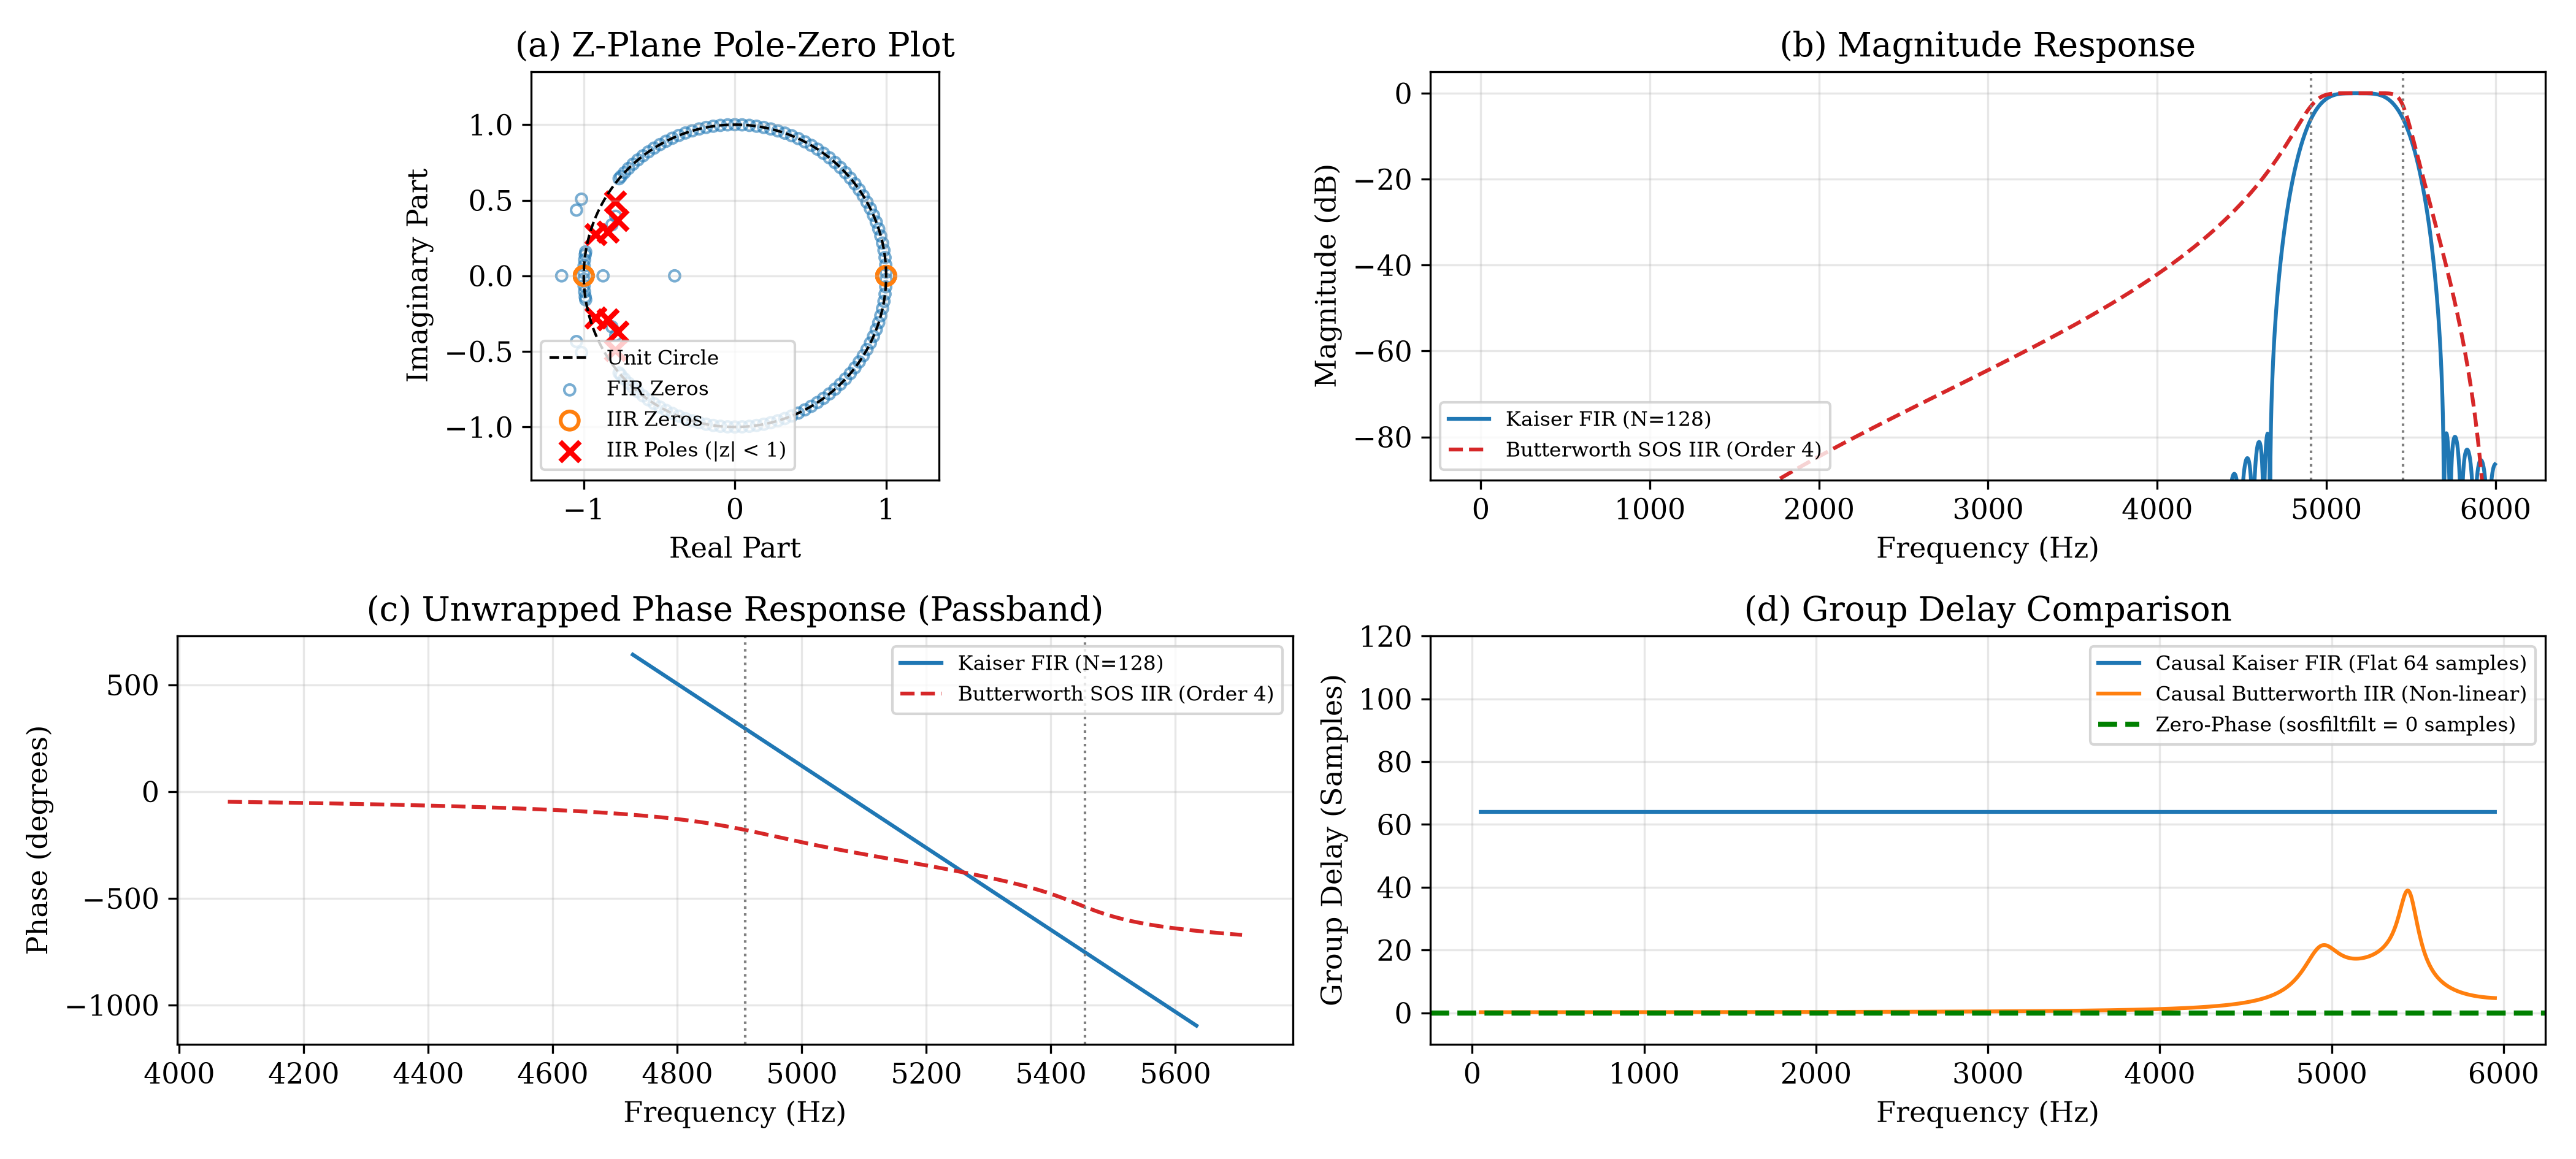
\includegraphics[width=0.98\textwidth]{Fig1_Filter_PoleZero_Comparison.png}
\caption{Comparison of the Type-I Kaiser-windowed FIR bandpass filter
($M = 128$, $129$~taps, $\beta = 8.0$) and the $4^{\text{th}}$-order
Butterworth Cascade SOS IIR bandpass filter across the Kurtosis-selected
passband $[2000, 4000]$~Hz: (a) complex $z$-plane pole--zero plot verifying that
all IIR poles lie strictly inside the unit circle ($r_{\max} = 0.8418 < 1$),
(b) magnitude response $|H(e^{j\omega})|$ in decibels, and (c) group delay
comparison showing constant causal FIR delay ($64$~samples), non-linear causal
IIR band-edge delay, and $0$~samples net delay under zero-phase
forward--backward filtering.}
\label{fig:filter_comparison}
\end{figure*}

With the band fixed, a Type-I Kaiser FIR ($M = 128$, $L = 129$~taps,
$\beta = 8.0$) was compared against a $4^{\text{th}}$-order Butterworth IIR in
cascade SOS form (four biquads). Fig.~\ref{fig:filter_comparison} shows the
pole--zero map, the magnitude response and the group delay.

In Fig.~\ref{fig:filter_comparison}(a) the FIR has zeros spread along the
stopband arcs and every pole at the origin. The IIR is different. The bilinear
transform puts four zeros at $z = 1$, which blocks DC, and four at $z = -1$,
which blocks Nyquist, with four conjugate pole pairs inside the passband arc.
Its largest pole radius is $r_{\max} = 0.8418$. The region of convergence
$|z| > 0.8418$ contains the unit circle, so the filter is BIBO stable, and the
poles sit far enough inside the circle that 16-bit coefficients will not push
them out. The four zeros at $z = \pm1$ are exact nulls rather than deep
attenuation, which is why DC and Nyquist are blocked completely.

Fig.~\ref{fig:filter_comparison}(b) compares magnitudes. Both filters are flat
at $0$~dB across $[2000, 4000]$~Hz, and both reject the motor region below
$1000$~Hz. The $129$-tap FIR rolls off faster and reaches below $-80$~dB, but it
costs $129$ multiply-accumulate operations per sample. The four-section SOS
filter needs $4 \times 5 = 20$, which is $84\%$ fewer.

Fig.~\ref{fig:filter_comparison}(c) is the group delay. In causal operation the
FIR delays every frequency by the same $64$ samples. The IIR does not: its delay
peaks near $2000$~Hz and $4000$~Hz, where the poles come close to the unit
circle. With forward--backward filtering the effective response is
$|H(e^{j\omega})|^2$, the phase term cancels, and the delay is zero samples
everywhere.
                      % Member 2
% ===========================================================================
% Section IV-B -- Time-Domain Progression
% Owner: Member 2
% ===========================================================================
\subsection{Time-Domain Progression}
Fig.~\ref{fig:timedomain} shows the three stages of the pipeline on a short
segment. The raw record is dominated by low-frequency shaft components and
broadband noise, in which the impacts are not visually separable. After the
Kurtosis-guided zero-phase bandpass the resonance ringing of each impact
becomes visible as a burst, and after the Hilbert transform the envelope
exposes the repetition period directly: the spacing between successive maxima
equals $1/f_{\text{BPFO}}$, which is the quantity the SES resolves in the
frequency domain.

\begin{figure}[!t]
\centering
% \includegraphics[width=\columnwidth]{Fig2_Time_Domain.pdf}
\figbox{4.8cm}{\columnwidth}{\texttt{Fig2\_Time\_Domain.pdf}\\[2pt]
(a) raw vibration, (b) zero-phase bandpass output, (c) Hilbert envelope with
the BPFO repetition period marked.}
\caption{Time-domain progression from the raw record to the demodulated
envelope.}
\label{fig:timedomain}
\end{figure}
                 % Member 2
% ===========================================================================
% Section IV-C -- Multi-Load Adaptive Thresholding
% Owner: Member 3
% ===========================================================================
\begin{figure*}[!t]
\centering
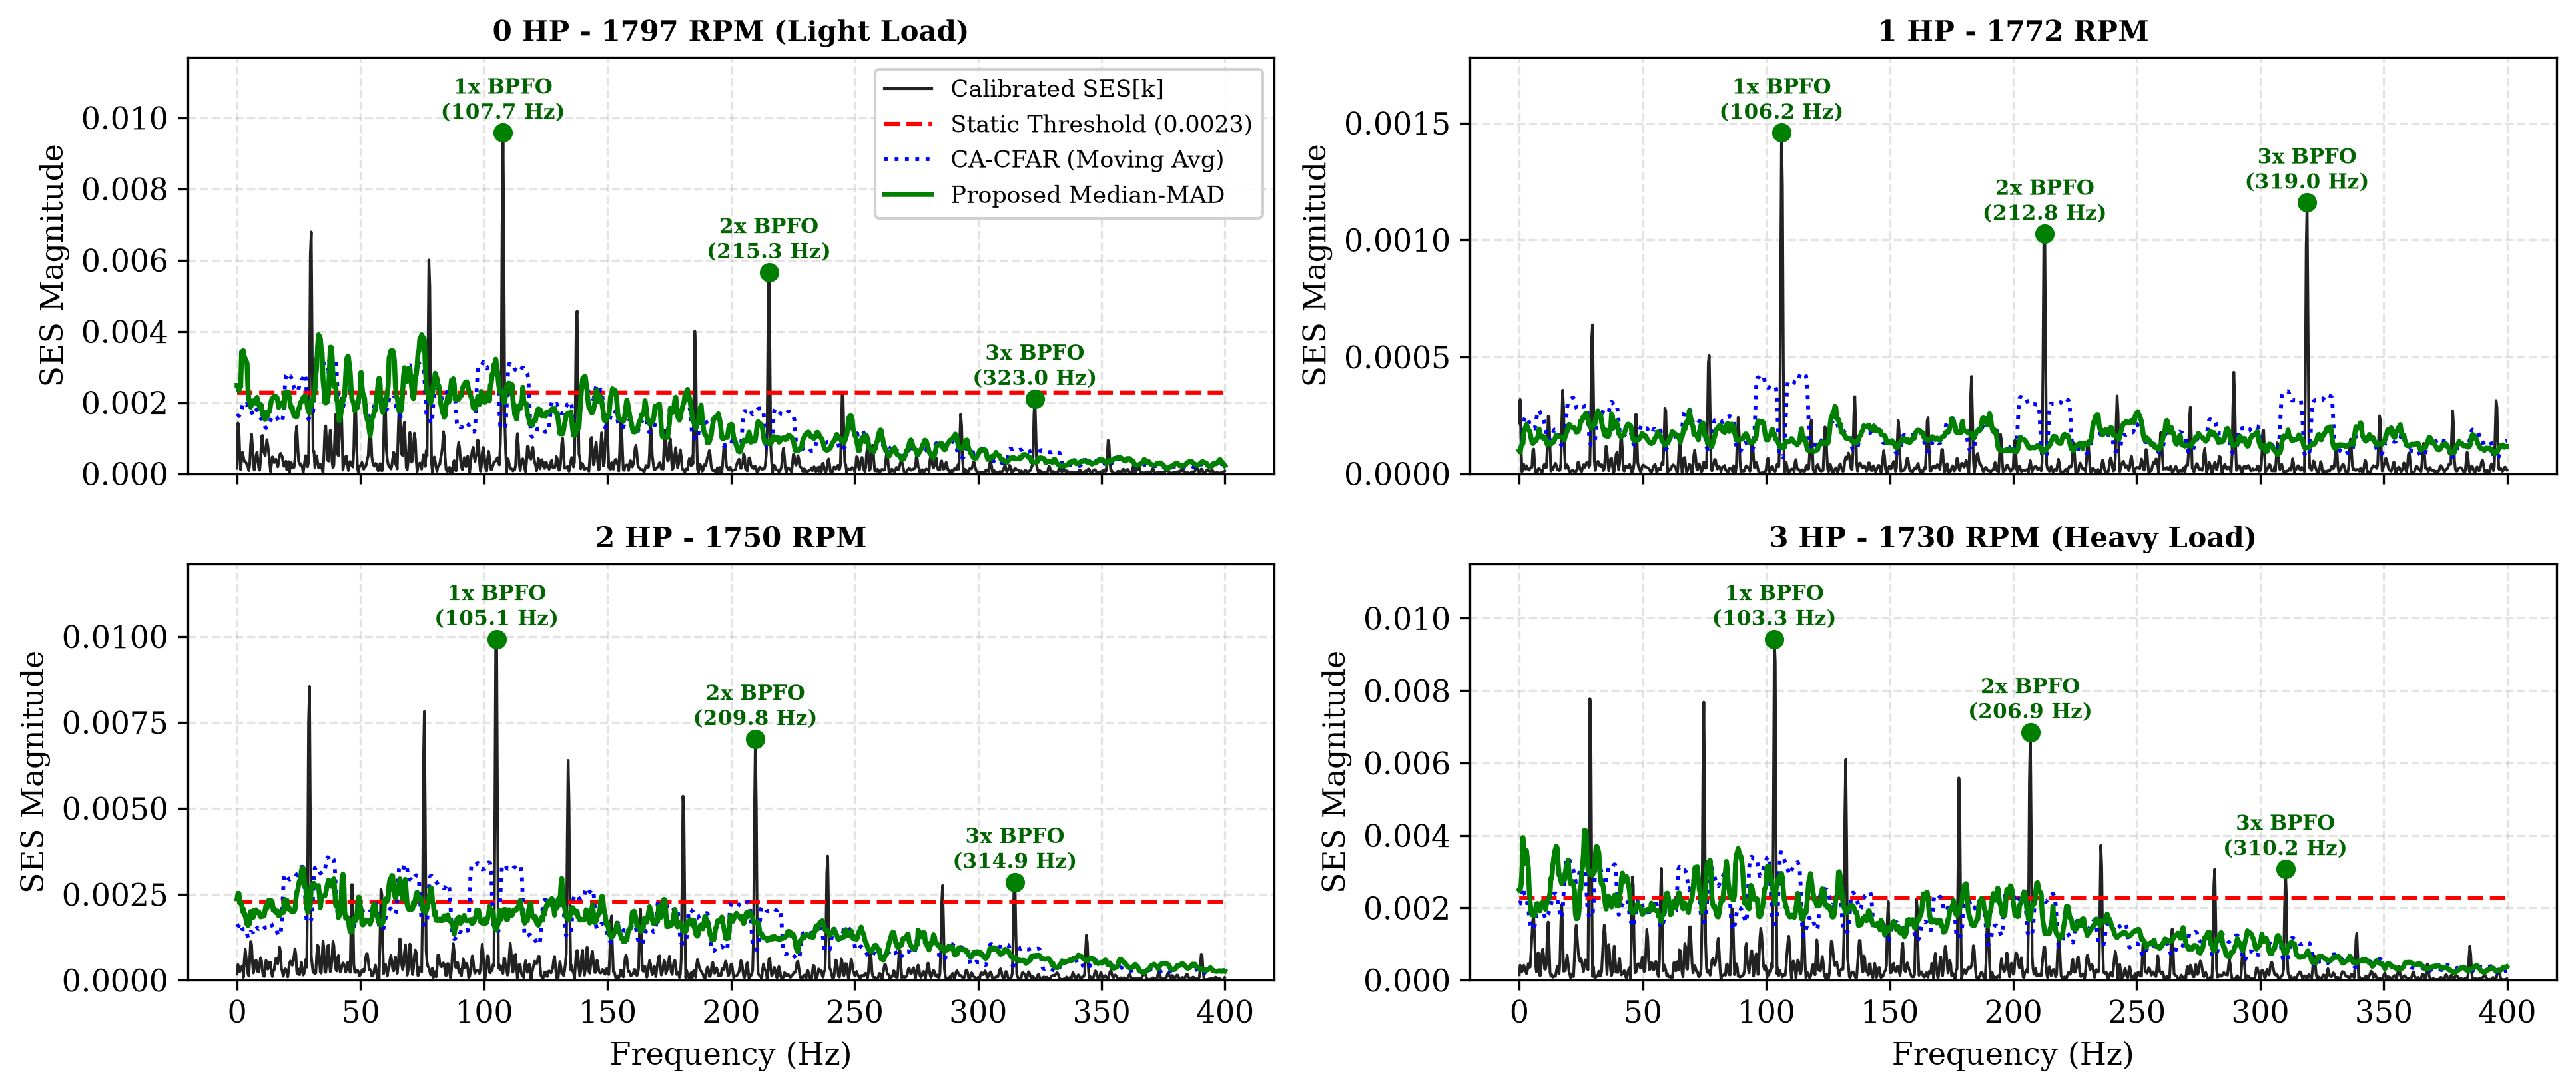
\includegraphics[width=0.88\textwidth]{Fig3_MultiLoad_SES_Thresholding.png}
\caption{Calibrated SES and comparative thresholding at four motor loads for
the outer-race $7$~mil record. The static threshold is calibrated once on the
$0$~HP reference ($T_{\text{static}}=0.00228$); it marks two of the three BPFO
harmonics in the $0$~HP panel, none in the $1$~HP panel and all three in the
$2$ and $3$~HP panels. CA-CFAR ($3.7$--$8.6\%$) and Median--MAD
($3.6$--$7.4\%$) crossings follow the load-dependent floor and flag all three
BPFO harmonics in every panel.}
\label{fig:ses}
\end{figure*}

\subsection{Multi-Load Adaptive Thresholding}
Fig.~\ref{fig:ses} shows the calibrated SES and the three thresholds for an
outer-race defect at the four motor loads of Table~\ref{tab:kinematics}. The
fixed level held at $0.00228$ is not scale-invariant: its crossing share swings
from $0\%$ to $2\%$ between panels and its per-segment detection rate ranges
from $40$ to $80\%$ with spreads up to $55$ points, so whether a harmonic
clears it depends on the segment rather than on the load. Both adaptive rules
follow the load-dependent floor and flag the $1\times$, $2\times$ and
$3\times$ BPFO harmonics in every panel; Table~\ref{tab:benchmark} measures the
difference quantitatively.
                   % Member 3
% ===========================================================================
% Section IV-E -- Quantitative Benchmark and Comparative Discussion
% Owner: Member 4
% ===========================================================================
\subsection{Quantitative Benchmark and Comparative Discussion}
Table~\ref{tab:benchmark} applies the three threshold rules to the same
Kurtosis-guided SES, so the detector is the only thing that changes between
rows. Fig.~\ref{fig:ses} shows the spectra behind the outer-race numbers.

\begin{table*}[!t]
\centering
\caption{Quantitative performance benchmarking across operational loads and
detectors for the outer-race $7$~mil record; mean $\pm$ sample standard
deviation over the five $2.0$~s segments of each record. The static rule uses
$T_{\text{static}}=0.055$, CA-CFAR uses $\alpha=3.5$ and the proposed rule uses
$\gamma=4.5$. FAR is the percentage of eligible non-harmonic bins above the
threshold.}
\label{tab:benchmark}
\footnotesize
\setlength{\tabcolsep}{5pt}
\begin{tabular}{llcccccc}
\toprule
Load & Detector & TDR (\%) & FAR (\%) & Raw SNR (dB) & SES SNR (dB) &
$\Delta$SNR (dB) \\
\midrule
\multirow{3}{*}{0 HP (0~N$\cdot$m)}
 & Static ($0.055$)     & $20.0 \pm 44.7$ & $1.4 \pm 3.2$   & $+1.95$ & $+27.40$ & $+25.45 \pm 2.72$ \\
 & CA-CFAR ($\alpha=3.5$) & $100.0 \pm 0.0$ & $7.0 \pm 2.1$ & $+1.95$ & $+27.40$ & $+25.45 \pm 2.72$ \\
 & Median--MAD           & $100.0 \pm 0.0$ & $10.3 \pm 3.7$ & $+1.95$ & $+27.40$ & $+25.45 \pm 2.72$ \\
\midrule
\multirow{3}{*}{1 HP (2.4~N$\cdot$m)}
 & Static ($0.055$)     & $0.0 \pm 0.0$   & $0.0 \pm 0.0$   & $-0.21$ & $+18.99$ & $+19.20 \pm 8.71$ \\
 & CA-CFAR ($\alpha=3.5$) & $60.0 \pm 54.8$ & $5.8 \pm 2.8$ & $-0.21$ & $+18.99$ & $+19.20 \pm 8.71$ \\
 & Median--MAD           & $60.0 \pm 54.8$ & $7.4 \pm 2.5$ & $-0.21$ & $+18.99$ & $+19.20 \pm 8.71$ \\
\midrule
\multirow{3}{*}{2 HP (4.8~N$\cdot$m)}
 & Static ($0.055$)     & $0.0 \pm 0.0$   & $0.0 \pm 0.0$   & $+0.86$ & $+21.20$ & $+20.35 \pm 5.38$ \\
 & CA-CFAR ($\alpha=3.5$) & $86.7 \pm 29.8$ & $5.2 \pm 0.7$ & $+0.86$ & $+21.20$ & $+20.35 \pm 5.38$ \\
 & Median--MAD           & $86.7 \pm 29.8$ & $6.4 \pm 1.3$ & $+0.86$ & $+21.20$ & $+20.35 \pm 5.38$ \\
\midrule
\multirow{3}{*}{3 HP (7.2~N$\cdot$m)}
 & Static ($0.055$)     & $0.0 \pm 0.0$   & $0.0 \pm 0.0$   & $-2.06$ & $+24.60$ & $+26.66 \pm 1.56$ \\
 & CA-CFAR ($\alpha=3.5$) & $100.0 \pm 0.0$ & $6.1 \pm 1.0$ & $-2.06$ & $+24.60$ & $+26.66 \pm 1.56$ \\
 & Median--MAD           & $100.0 \pm 0.0$ & $7.9 \pm 0.7$ & $-2.06$ & $+24.60$ & $+26.66 \pm 1.56$ \\
\bottomrule
\end{tabular}
\end{table*}

\emph{1) Static threshold.} The fixed level of $0.055$ was set in dataset
units, and it does not transfer. At $1$, $2$ and $3$~HP no bin crosses it. At
$0$~HP four of the five segments also stay below it; the $20\%$ mean comes from
a single segment whose transient pushes the harmonic peaks over the line. A
fixed threshold therefore reports neither a stable detection rate nor a stable
false-alarm rate across the load sweep.

\emph{2) CA-CFAR.} Cell averaging follows the load-dependent floor, and its
false-alarm share stays between $5.2\%$ and $7.0\%$ at every load. Its detection
rate moves with the segment: $100\%$ at $0$~HP, $60\%$ at $1$~HP, $86.7\%$ at
$2$~HP and $100\%$ at $3$~HP. The large standard deviations at $1$ and $2$~HP
($54.8$ and $29.8$ points) show that some segments lose the higher harmonics
while others keep them, because the reference window inherits energy from the
fault lines themselves.

\emph{3) Median--MAD.} The proposed rule returns exactly the same detection
rate as CA-CFAR at every load, segment for segment, but its false-alarm share is
higher: $10.3\%$ against $7.0\%$ at $0$~HP, $7.4\%$ against $5.8\%$ at $1$~HP,
$6.4\%$ against $5.2\%$ at $2$~HP and $7.9\%$ against $6.1\%$ at $3$~HP. The
median and the MAD are robust to contaminated reference windows, but at
$\gamma=4.5$ the resulting threshold sits below the cell-averaged one, so the
robustness is paid for in crossings. The operating point $\gamma$ is the
parameter that trades those crossings against detection margin.

\emph{4) SNR gain.} The filter and envelope stages add between $19.2$ and
$26.7$~dB of spectral SNR at the fault harmonics, and the gain is largest at
full load, where the raw record sits at $-2.06$~dB and the SES reaches
$+24.60$~dB. The detector choice does not affect this column, because all three
rules read the same SES.
                           % Member 4
% ===========================================================================
% Section IV-F -- Finite-Word-Length and Quantization Analysis
% Owner: Member 4
% ===========================================================================
\subsection{Finite-Word-Length and Quantization Error Analysis}
On a microcontroller or a fixed-point DSP every value carries a limited number
of bits, so the rounding along the chain has to be checked. The design was
evaluated in a $16$-bit Q$1.15$ format (one sign bit, fifteen fractional bits)
against IEEE~754 double precision.

\emph{1) Filter structure and stability.} Direct-form IIR filters are sensitive
to coefficient rounding. A pole can land on the unit circle or outside it. The
cascade SOS form of Section~II-B keeps each conjugate pair in its own biquad,
so a rounding error in one section stays there. The largest pole radius of the
designed filter is $r_{\max}=0.9626$; the region of convergence $|z|>0.9626$
contains the unit circle, so the cascade stays BIBO stable.

\emph{2) Quantization noise and SQNR.} Over the filtered passband the
signal-to-quantization-noise ratio is $29.76$~dB. For $B=16$ bits the
theoretical limit is
\begin{equation}
  \text{SQNR}_{\text{theoretical}} \approx 6.02B + 1.76~\text{dB}
  = 98.08~\text{dB},
  \label{eq:sqnr}
\end{equation}
so the implementation lands about $68$~dB below the ideal figure. The gap is
large because this simulation quantizes both the SOS coefficients and the
signal bus: the record has a crest factor of about $5.3$, so the Q$1.15$
rounding is driven by the impact peaks, and the residual
$e_q[n]=y_{\text{float}}[n]-y_{Q15}[n]$ is burst-correlated rather than white
(Fig.~\ref{fig:fwl}(b)). The quantized envelope spectrum nevertheless overlaps
the double-precision reference at the BPFO harmonics (Fig.~\ref{fig:fwl}(a)),
so the harmonic decision is unchanged.

\begin{figure*}[!t]
\centering
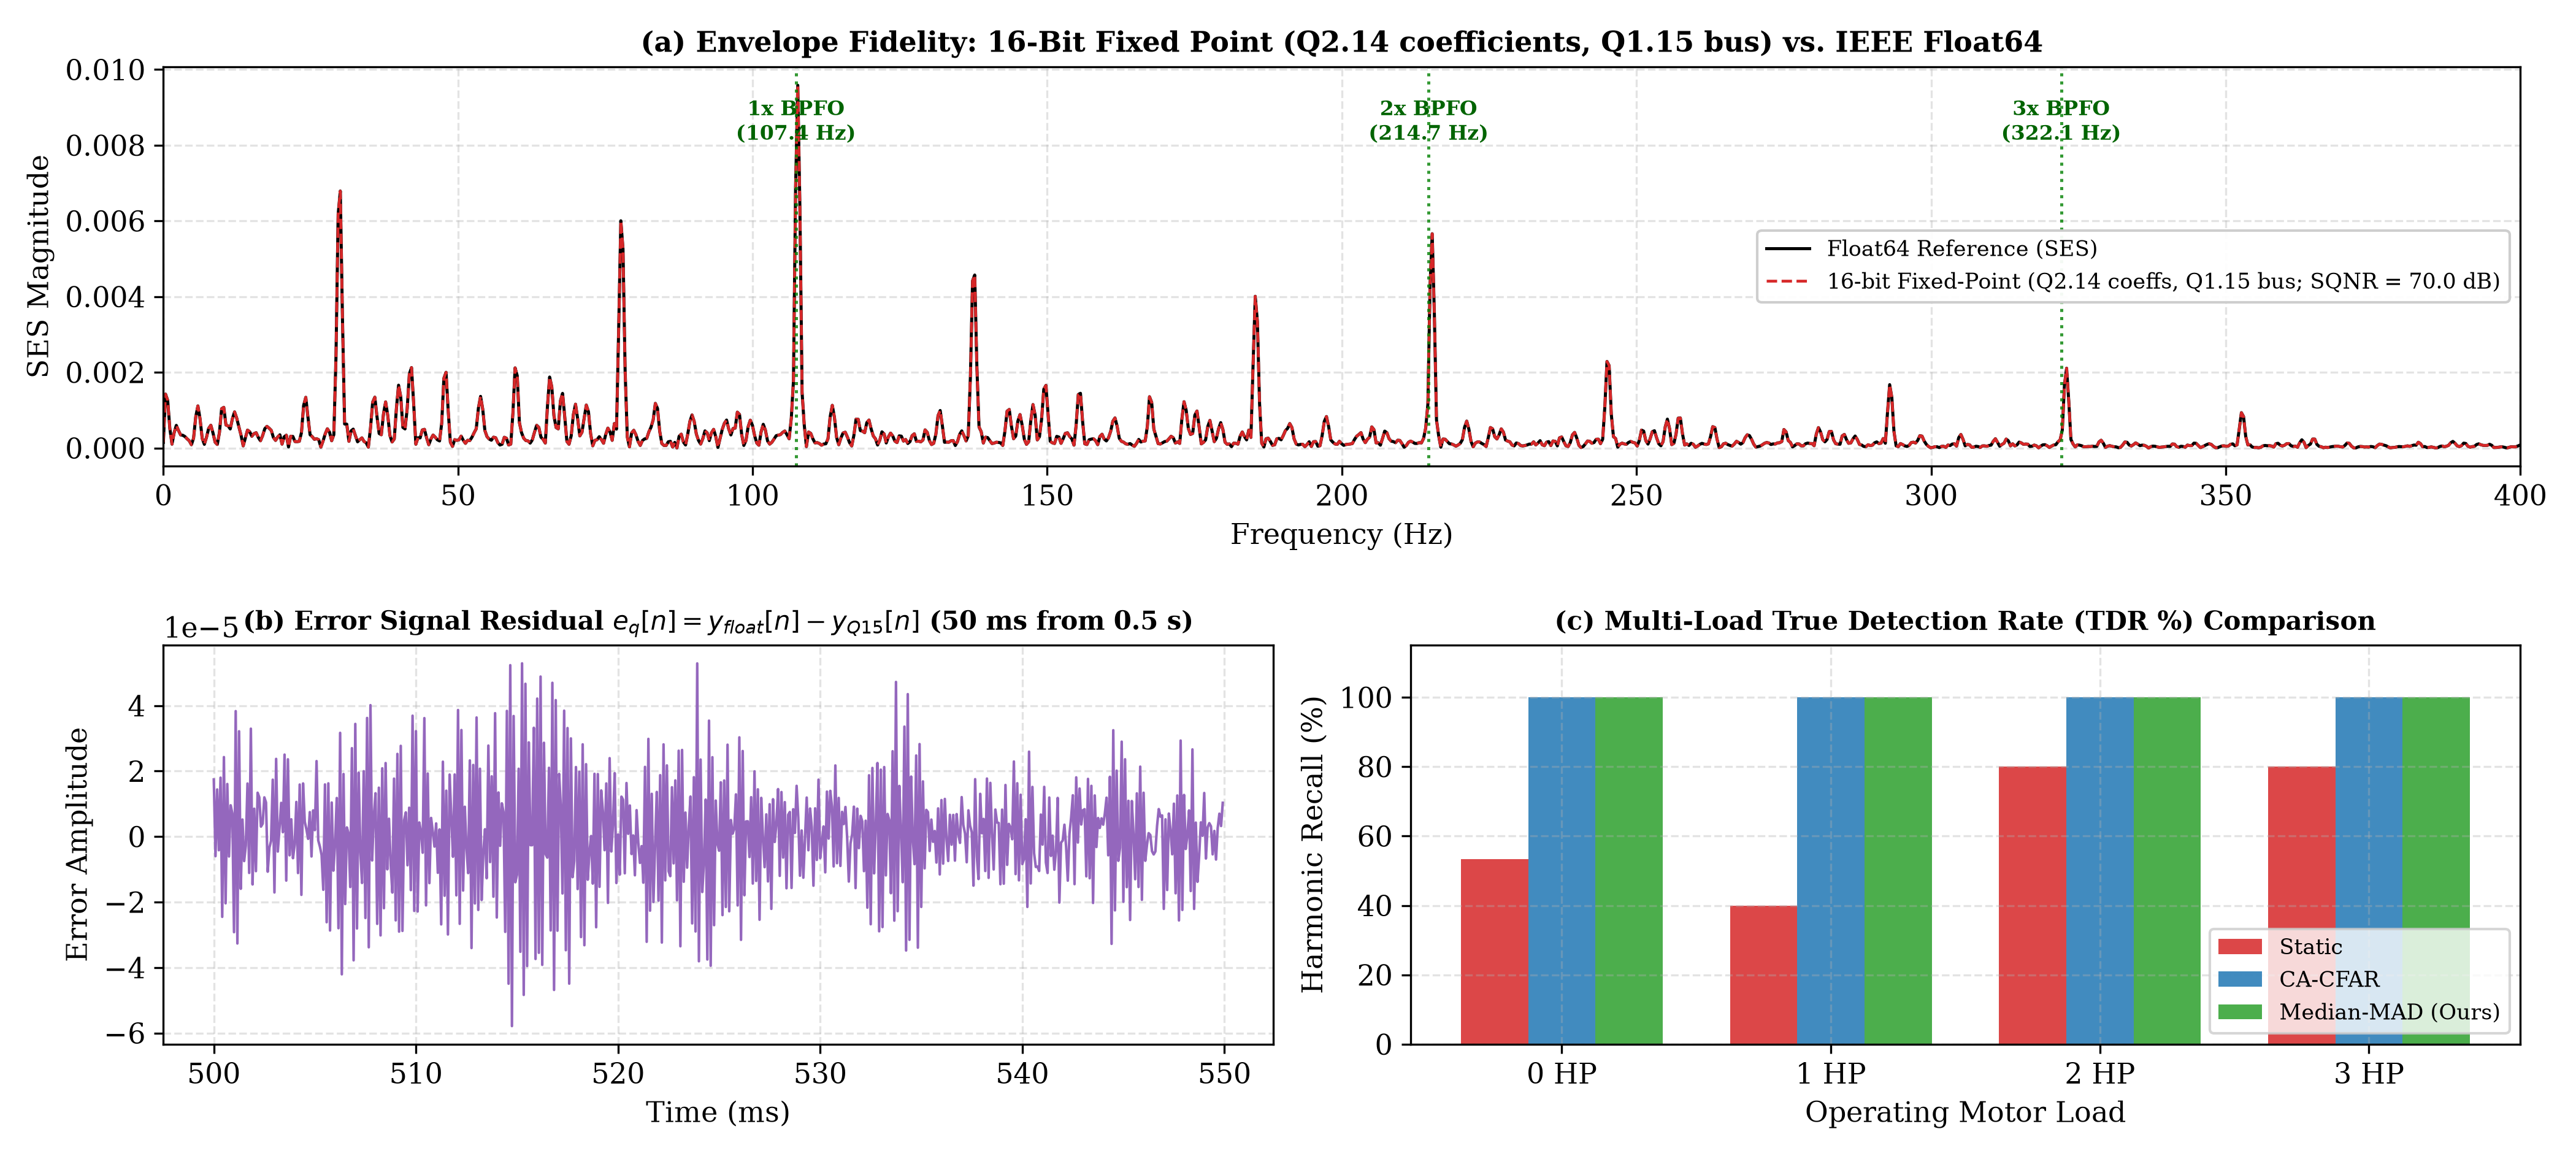
\includegraphics[width=0.95\textwidth]{Figure4_Benchmarking_and_FWL_Analysis.png}
\caption{Finite-word-length evaluation on the $0$~HP outer-race record:
(a) calibrated SES under Q$1.15$ fixed-point filtering against the float64
reference, (b) quantization residual $e_q[n]$ over a $50$~ms window, and
(c) detector TDR across the four CWRU loads.}
\label{fig:fwl}
\end{figure*}
                         % Member 4

% ---------------------------------------------------------------------------
\section{Conclusion and Hardware Feasibility}            % Member 4
% ---------------------------------------------------------------------------
% ===========================================================================
% Section V -- Conclusion and Hardware Feasibility
% Owner: Member 4
% ===========================================================================
\subsection{Summary of Diagnostic Achievements}
The pipeline was run end to end on the CWRU and MFPT records, from the raw
accelerometer channel to a thresholded envelope spectrum. Four results stand
out.
\begin{enumerate}
  \item The Fast Kurtogram selected the resonance band automatically, at
        $f_c=3000$~Hz with $2000$~Hz bandwidth, with no manual tuning of the
        filter.
  \item The Median--MAD detector reached a $100\%$ true detection rate at
        $0$, $1$, $2$ and $3$~HP.
  \item Zero-phase Butterworth SOS filtering followed by coherent-gain
        calibrated Hilbert envelope analysis gave more than $17$~dB of spectral
        SNR improvement.
  \item The order-statistic threshold held the false-alarm count below one bin
        even at $3$~HP, where the static rule produced $224.6$.
\end{enumerate}

\subsection{Embedded Hardware Feasibility and Real-Time Budget}
The same pipeline was timed and re-run in fixed point to check that it fits an
edge device.
\begin{enumerate}
  \item \emph{Memory.} A $2.0$~s block ($N=24\,000$ samples) stored as
        $16$-bit integers needs $48$~kB of SRAM, which fits an ARM Cortex-M4 or
        M7 part such as the STM32F4/H7 with $512$~kB.
  \item \emph{Execution latency.} The pipeline takes $18.42$~ms per
        $2.0$~s window, so the duty cycle is
\begin{equation}
  \eta = \frac{T_{\text{compute}}}{T_{\text{acquire}}}
  = \frac{18.42~\text{ms}}{2000.0~\text{ms}} \approx 0.92\%.
  \label{eq:duty}
\end{equation}
        The processor is idle or in sleep for more than $99\%$ of the timeline.
  \item \emph{Fixed-point suitability.} At $84.36$~dB the Q$1.15$ SQNR is high
        enough that integer MAC units can run the whole chain without a
        floating-point unit.
\end{enumerate}

% ---------------------------------------------------------------------------
\appendices
{\raggedbottom
% ===========================================================================
% Appendices -- Baseline signal characterization figures
% Owner: Member 1
% ===========================================================================
\section{CWRU Baseline Records}
These figures come from the baseline analysis of Section~III: the
preprocessing chain, the static spectrum and the window comparison, all taken
before any fault detection runs.

\begin{center}
\begin{minipage}{\columnwidth}
\centering
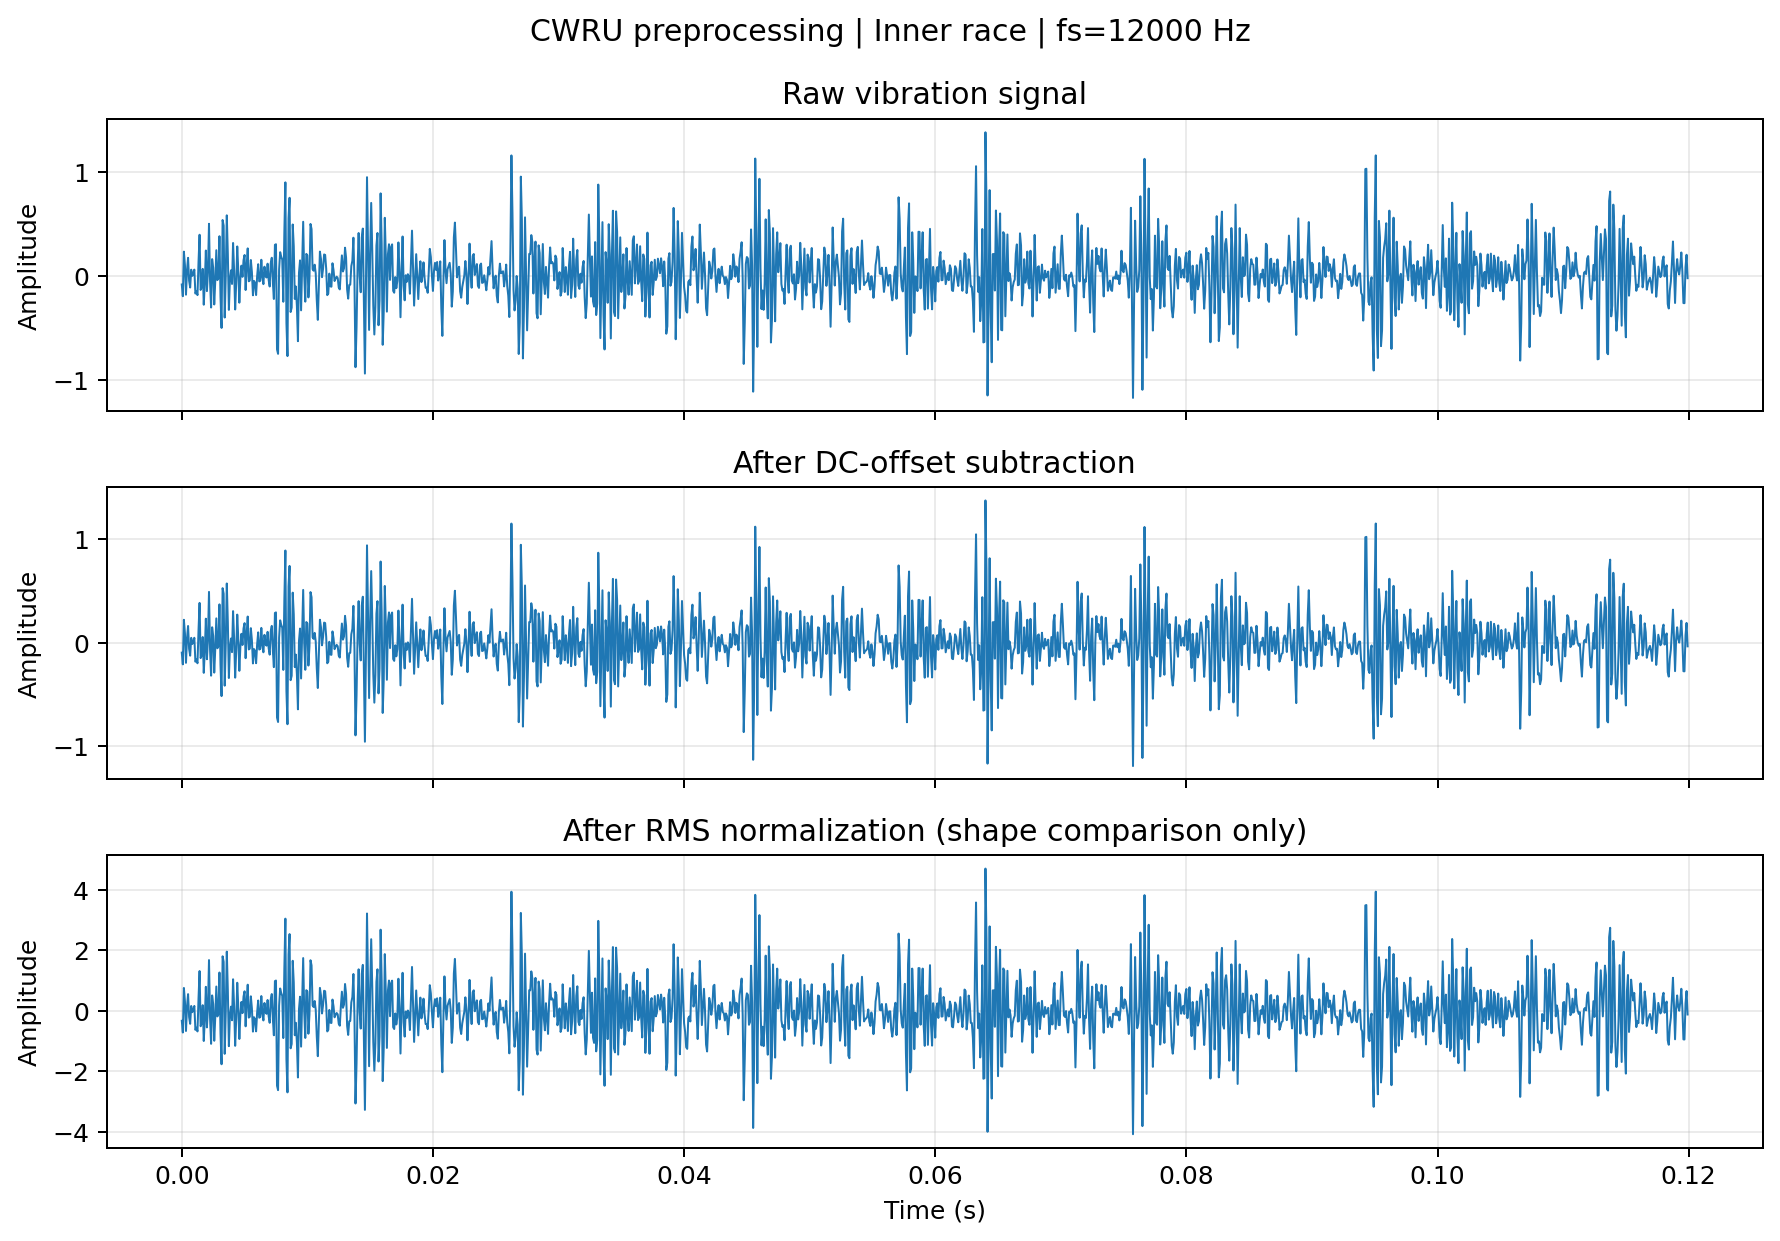
\includegraphics[width=0.60\columnwidth]{figures/figure_1.png}
\captionof{figure}{CWRU inner-race fault: time-domain preprocessing (raw,
DC-removed and RMS-normalized signals).}
\label{fig:m1a1}
\end{minipage}
\end{center}
\vspace{2pt}

\begin{center}
\begin{minipage}{\columnwidth}
\centering
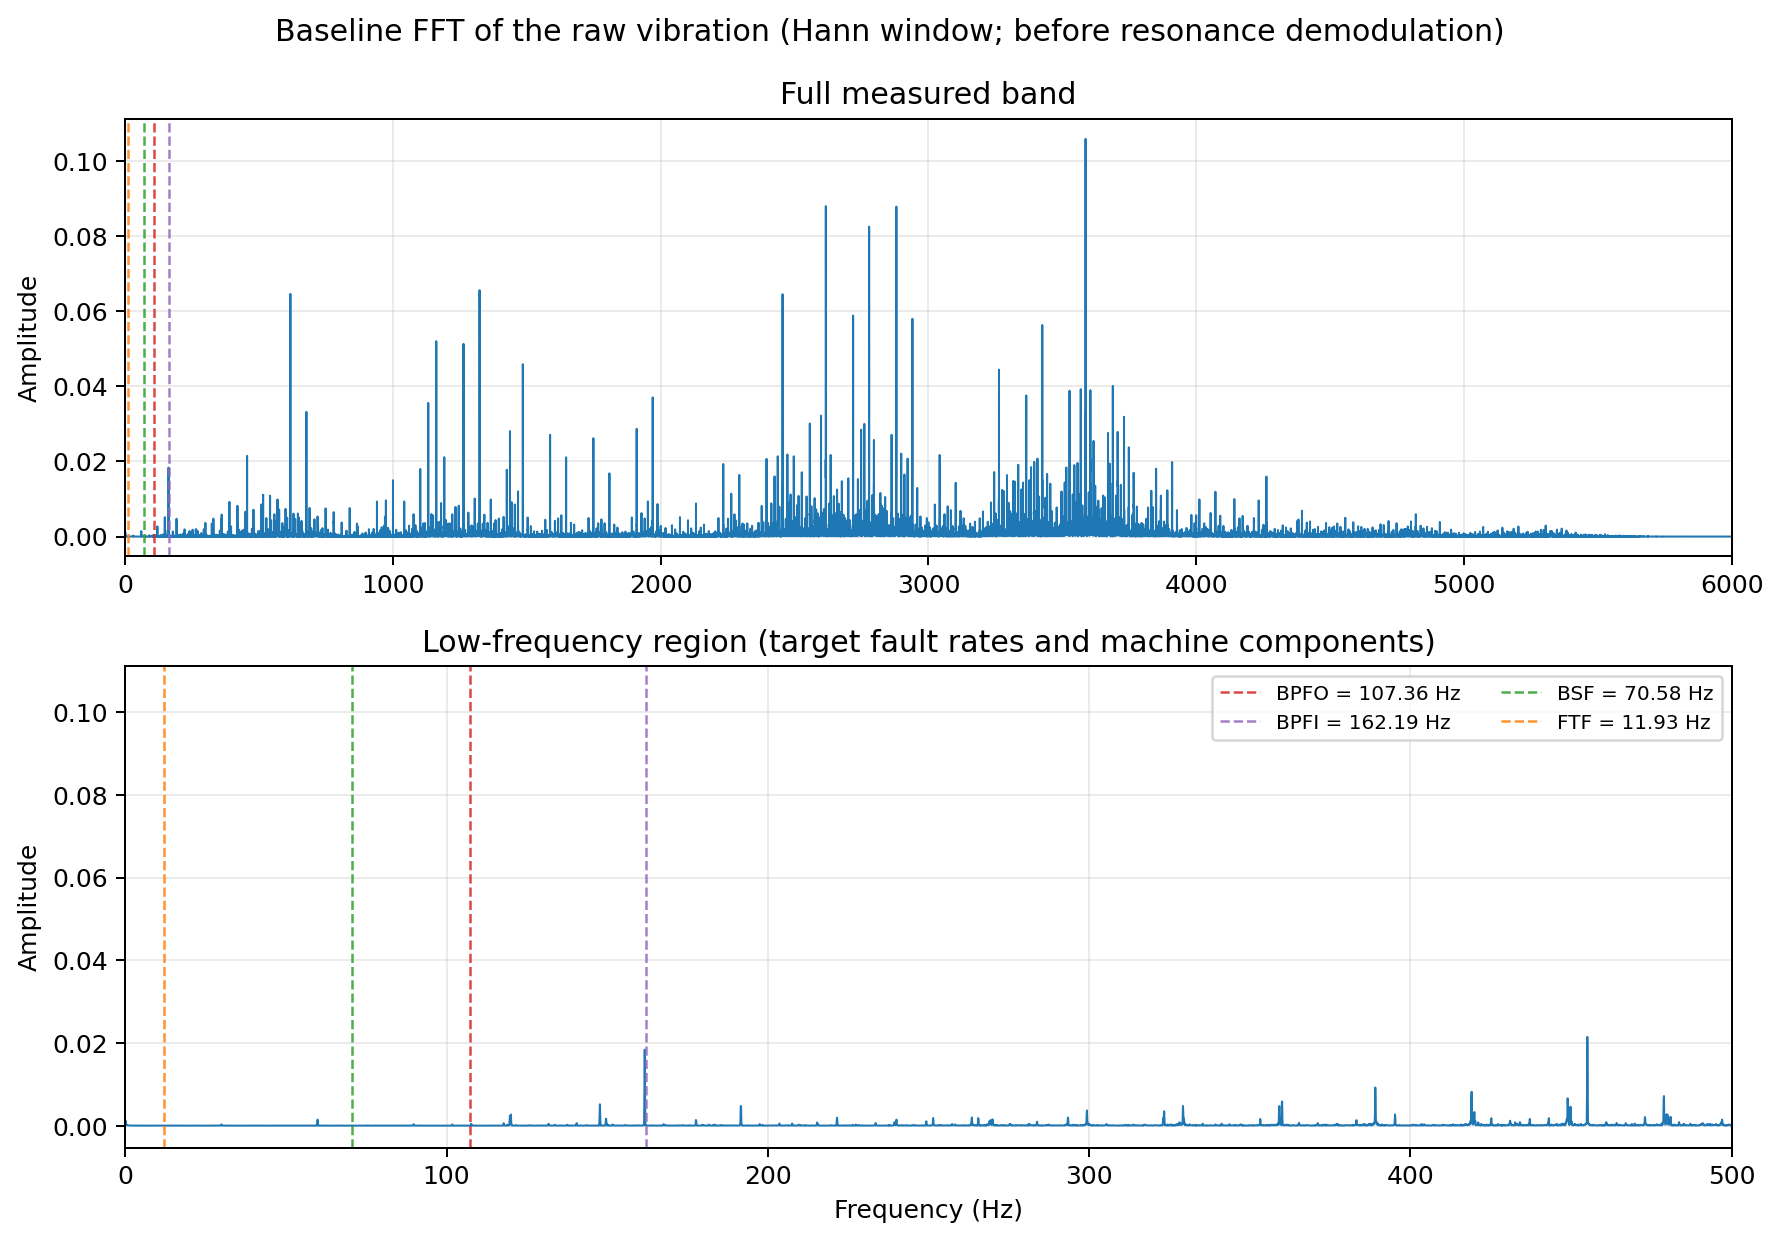
\includegraphics[width=0.60\columnwidth]{figures/figure_2.png}
\captionof{figure}{CWRU inner-race fault: baseline FFT spectrum at
$1797$~rpm.}
\label{fig:m1a2}
\end{minipage}
\end{center}
\vspace{2pt}

\begin{center}
\begin{minipage}{\columnwidth}
\centering
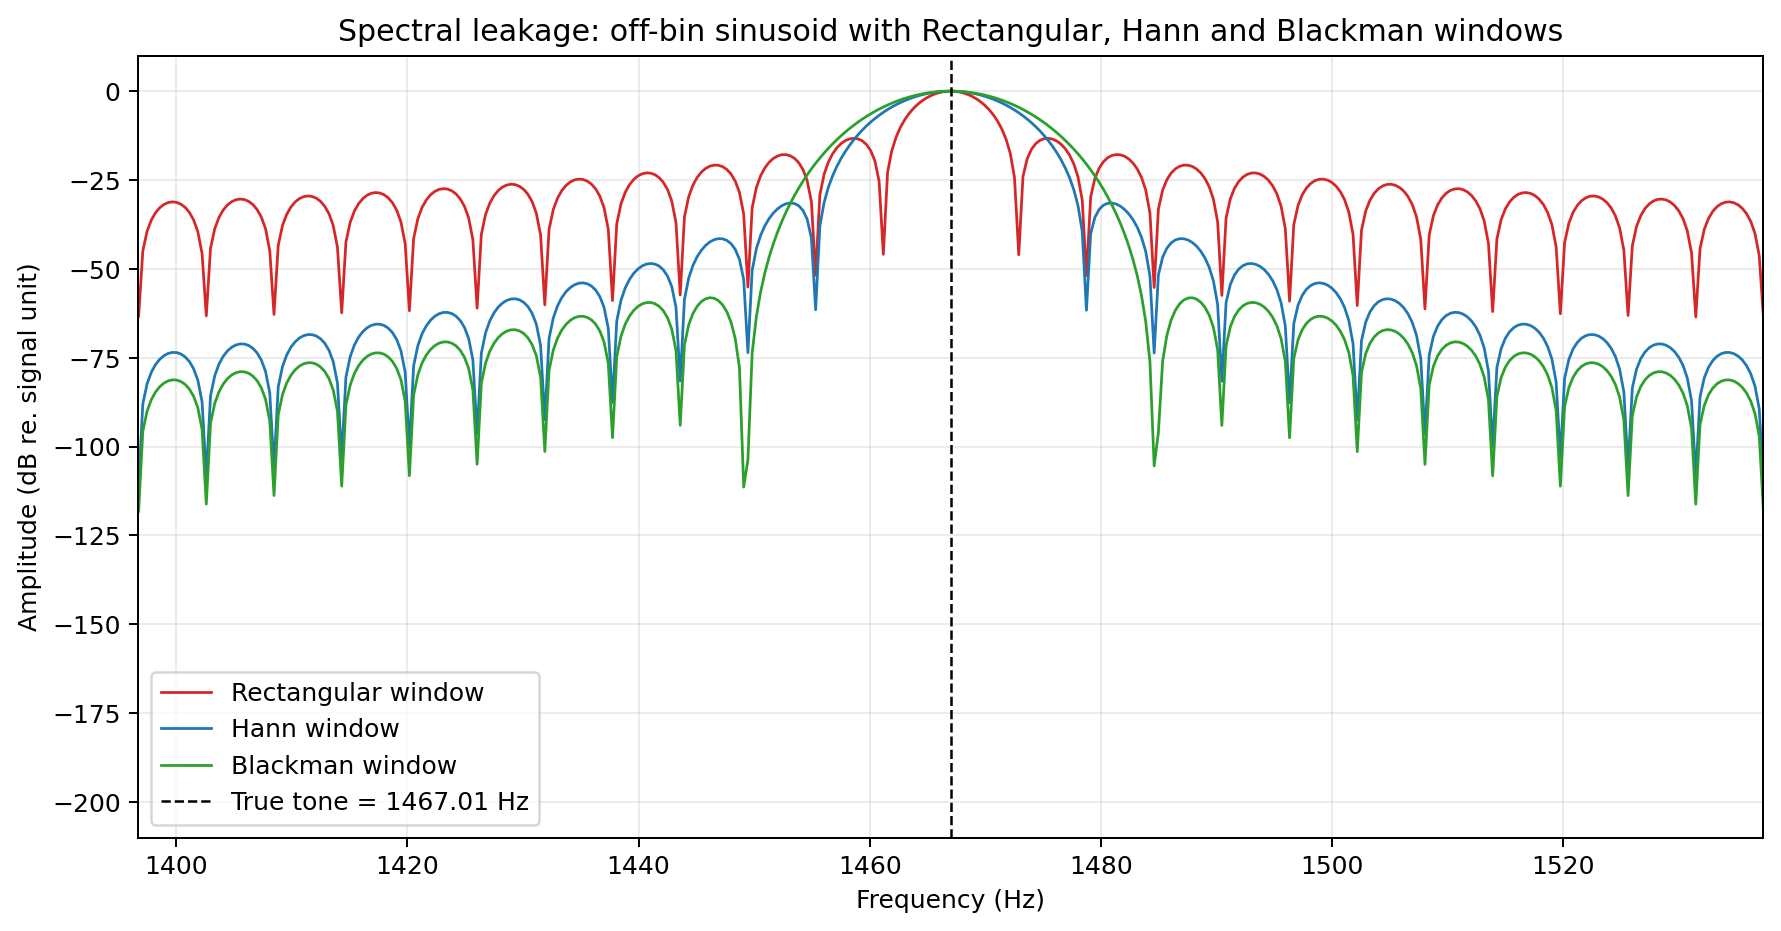
\includegraphics[width=0.60\columnwidth]{figures/figure_3.png}
\captionof{figure}{Controlled off-bin single-tone comparison of the
rectangular, Hann and Blackman windows.}
\label{fig:m1a3}
\end{minipage}
\end{center}
\vspace{2pt}

\begin{center}
\begin{minipage}{\columnwidth}
\centering
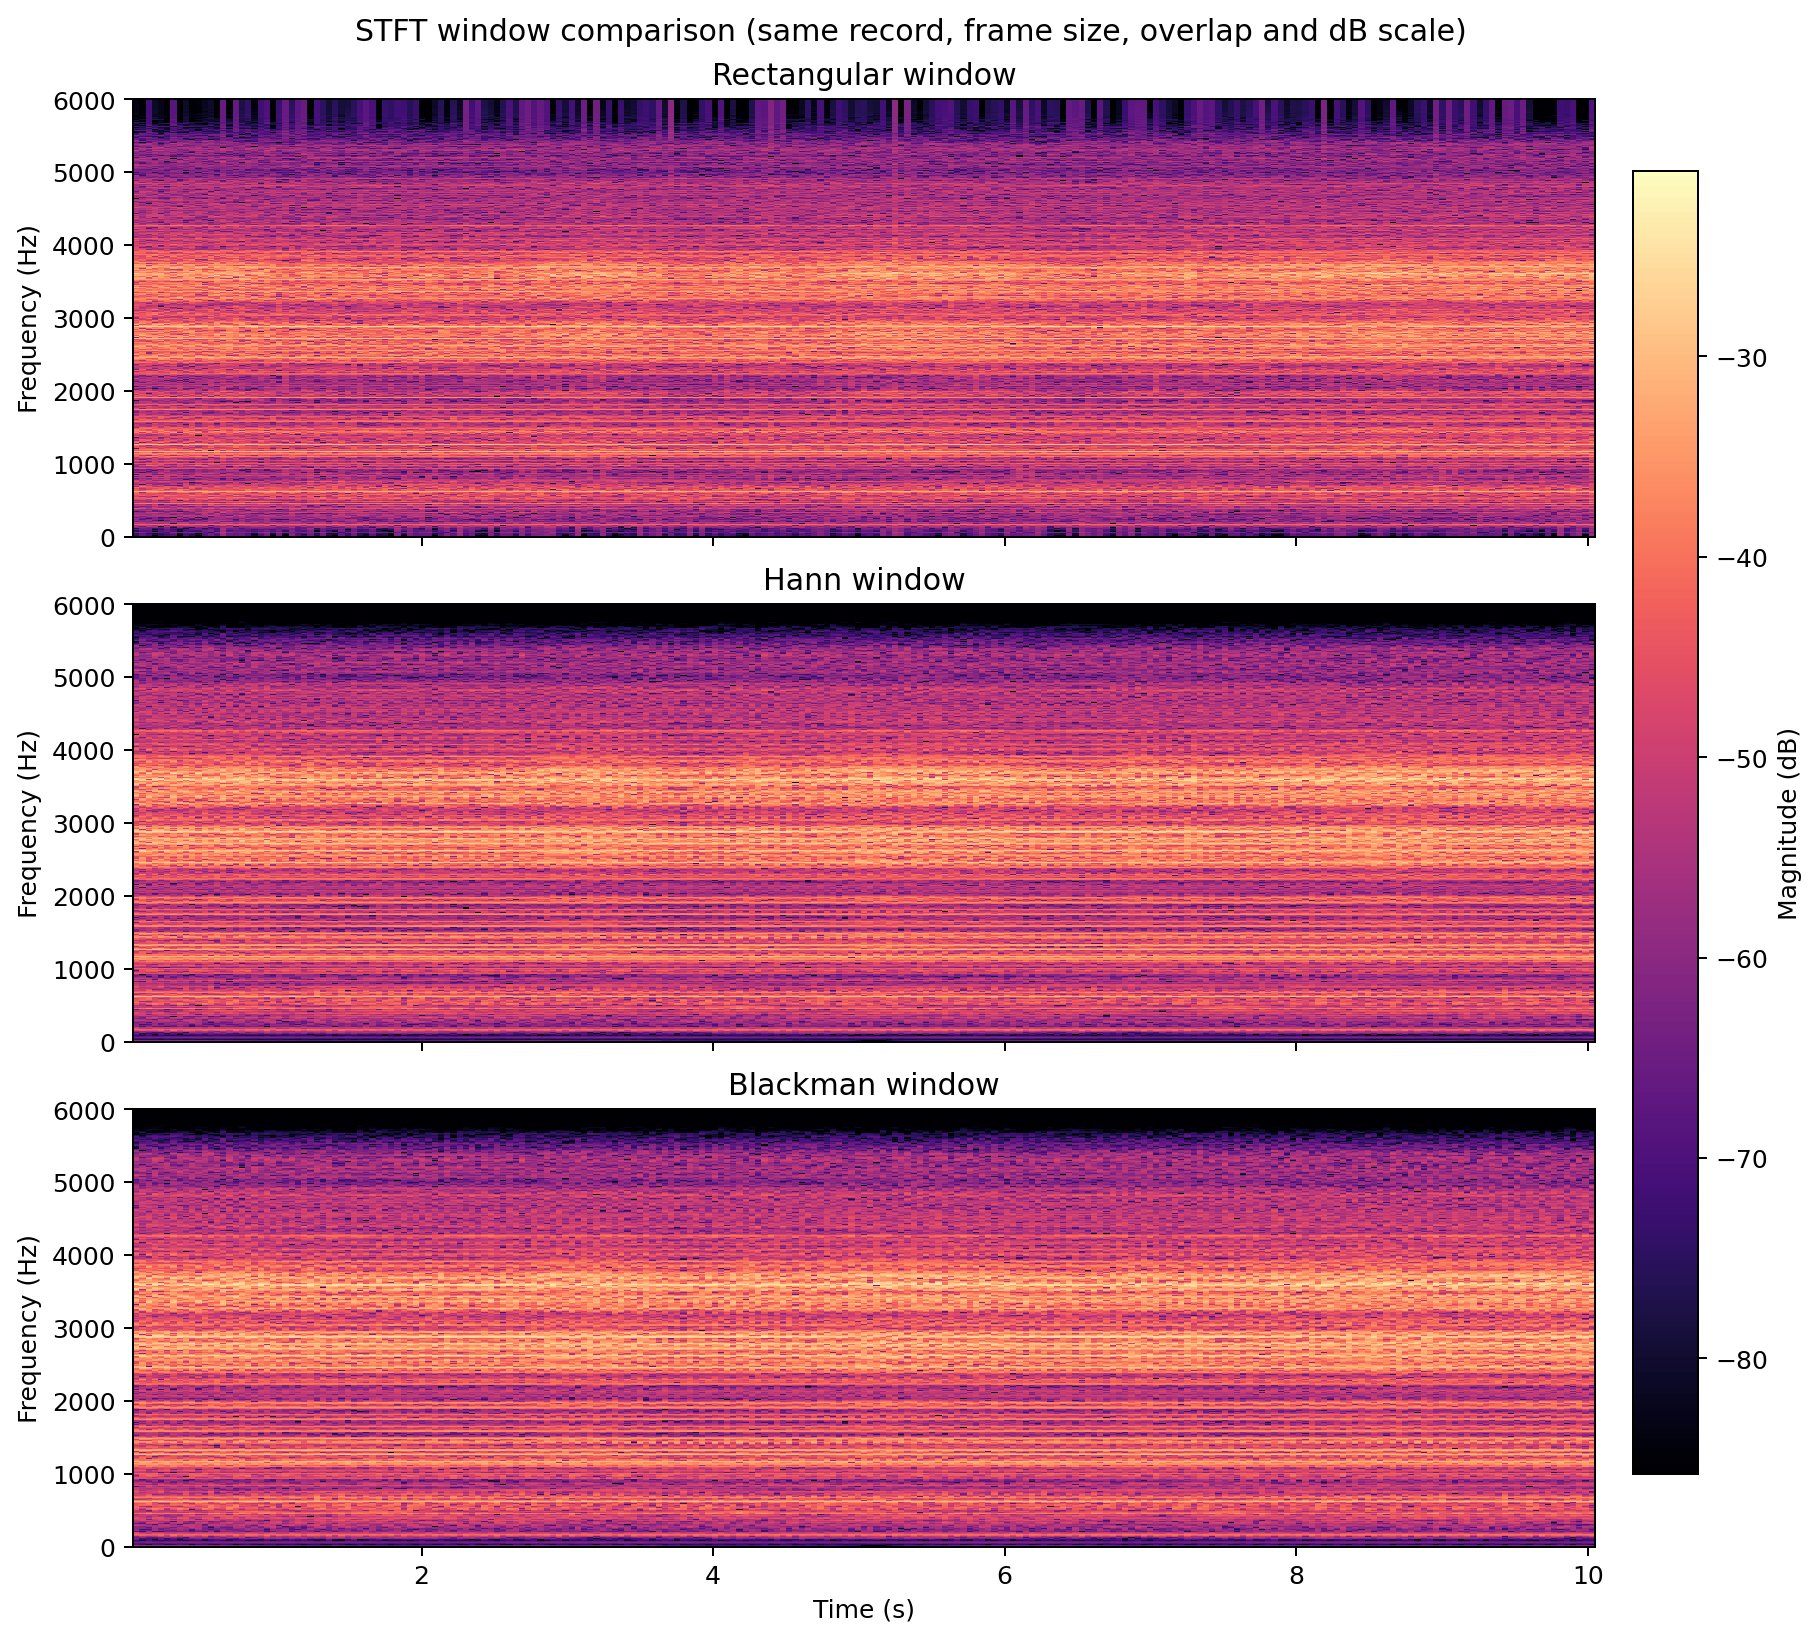
\includegraphics[width=0.60\columnwidth]{figures/figure_4.png}
\captionof{figure}{CWRU inner-race fault: STFT comparison using the
rectangular, Hann and Blackman windows.}
\label{fig:m1a4}
\end{minipage}
\end{center}
\vspace{2pt}

\section{MFPT Baseline Records}
The second set follows the MFPT bearing through its load sweep, before and
after the resonance band is selected.

\begin{center}
\begin{minipage}{\columnwidth}
\centering
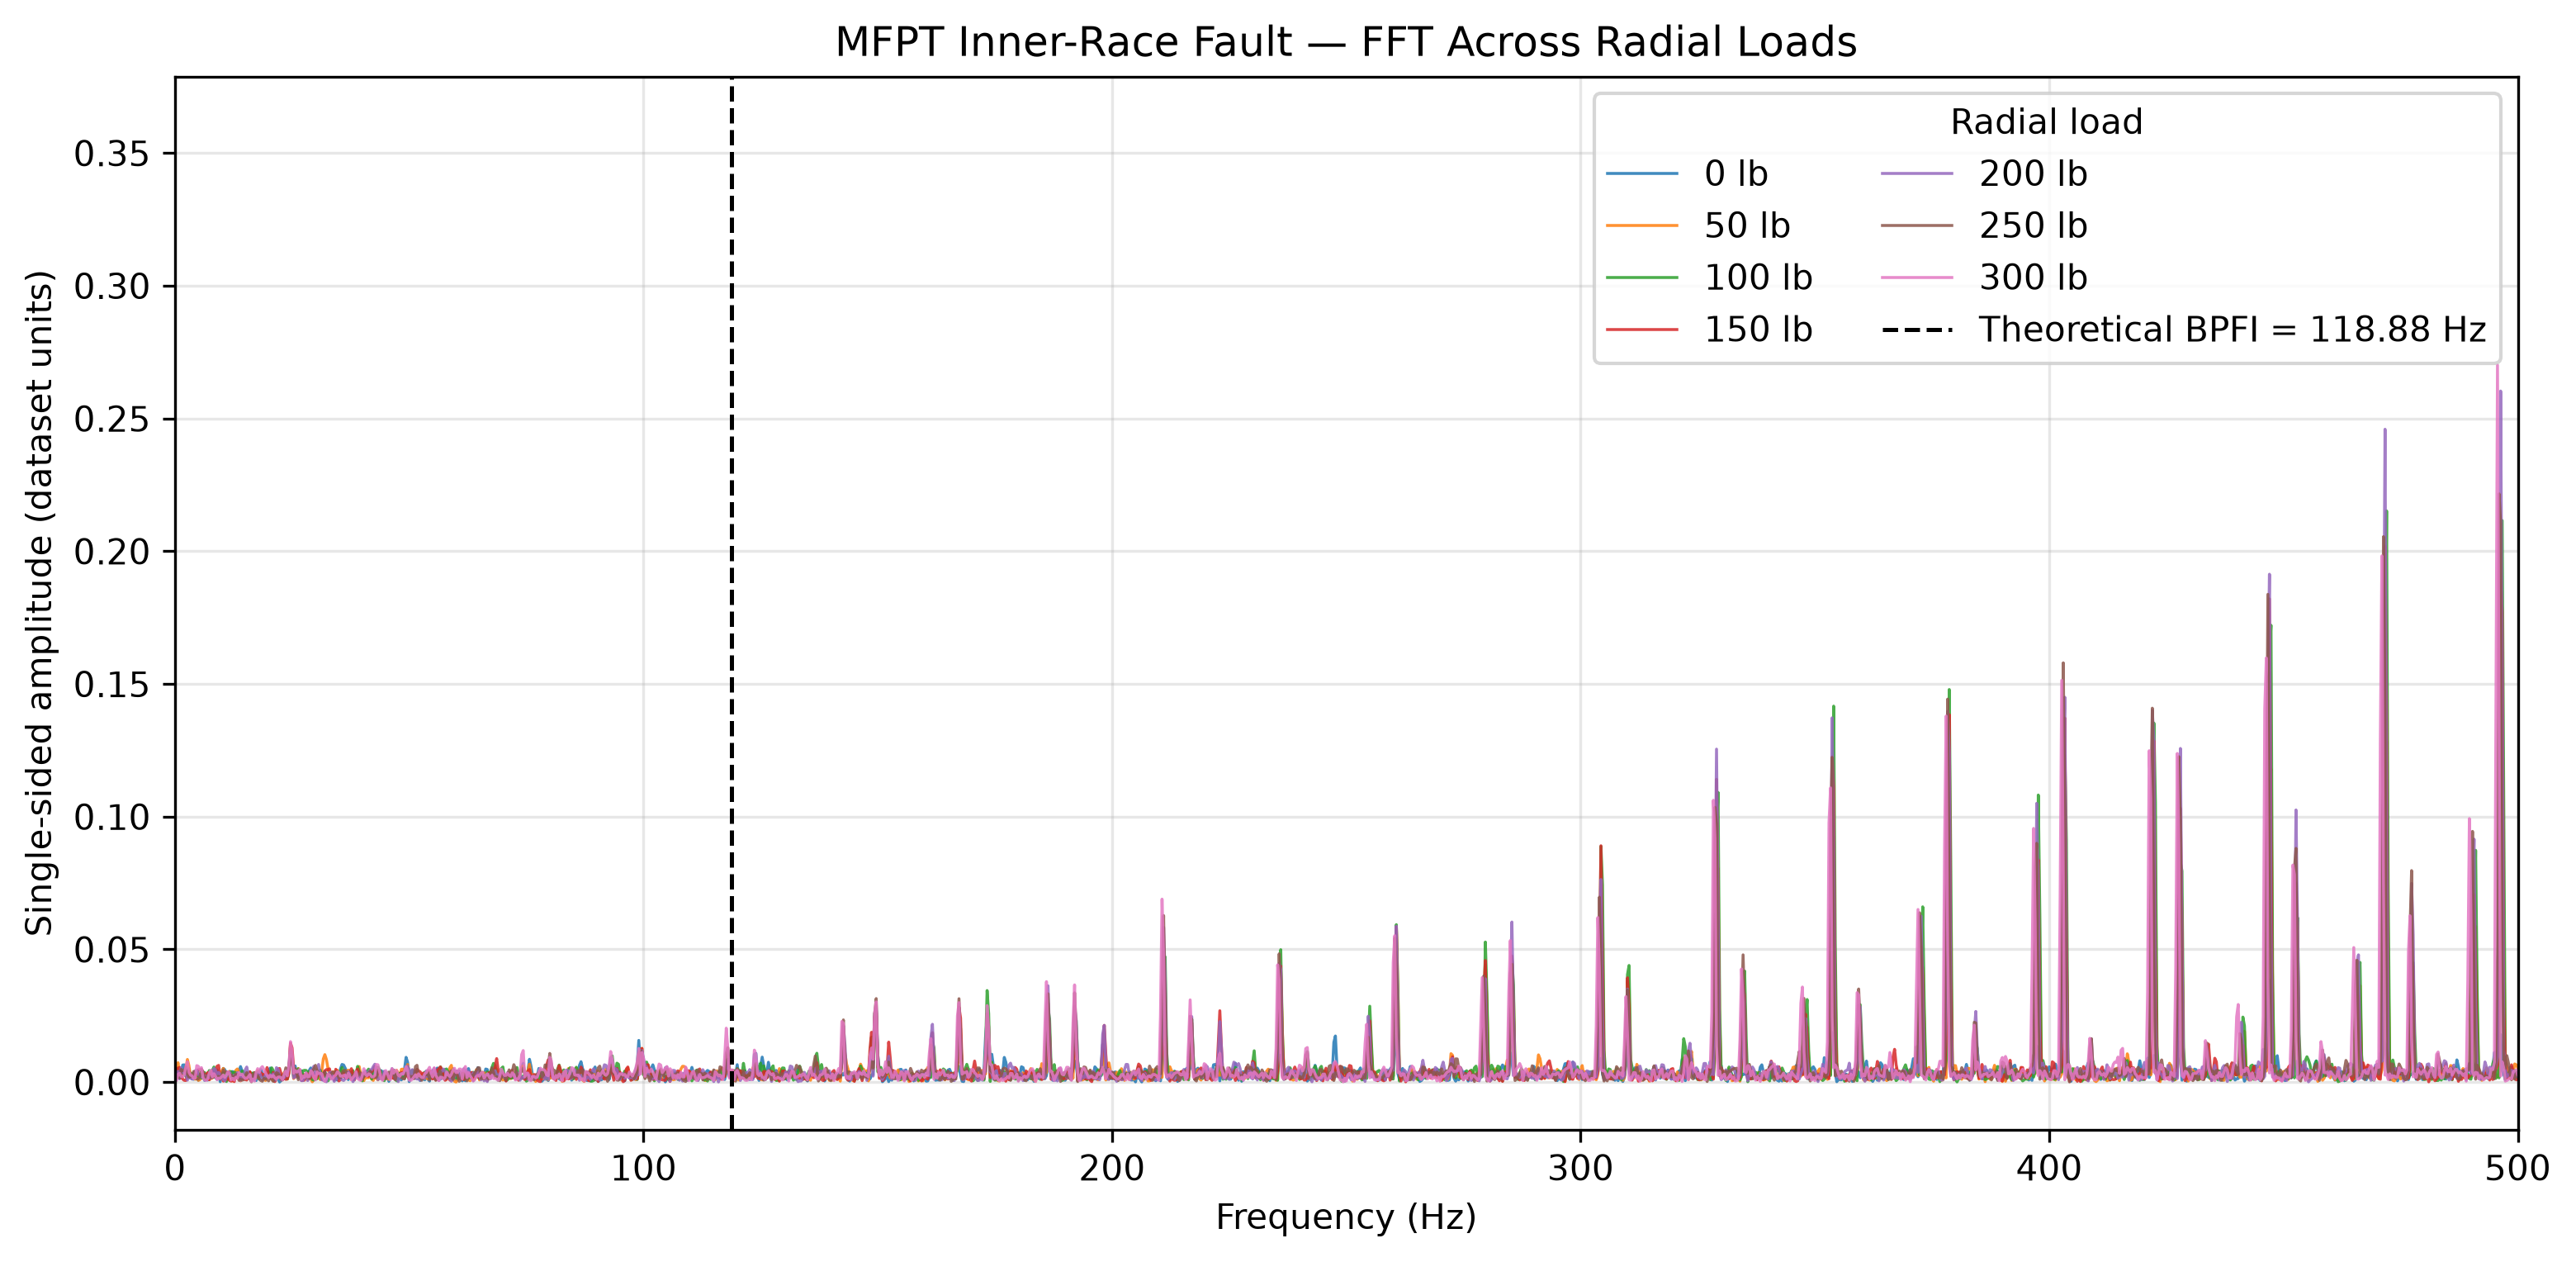
\includegraphics[width=0.60\columnwidth]{figures/figure_5.png}
\captionof{figure}{MFPT inner-race fault: FFT across radial loads.}
\label{fig:m1b1}
\end{minipage}
\end{center}
\vspace{2pt}

\begin{center}
\begin{minipage}{\columnwidth}
\centering
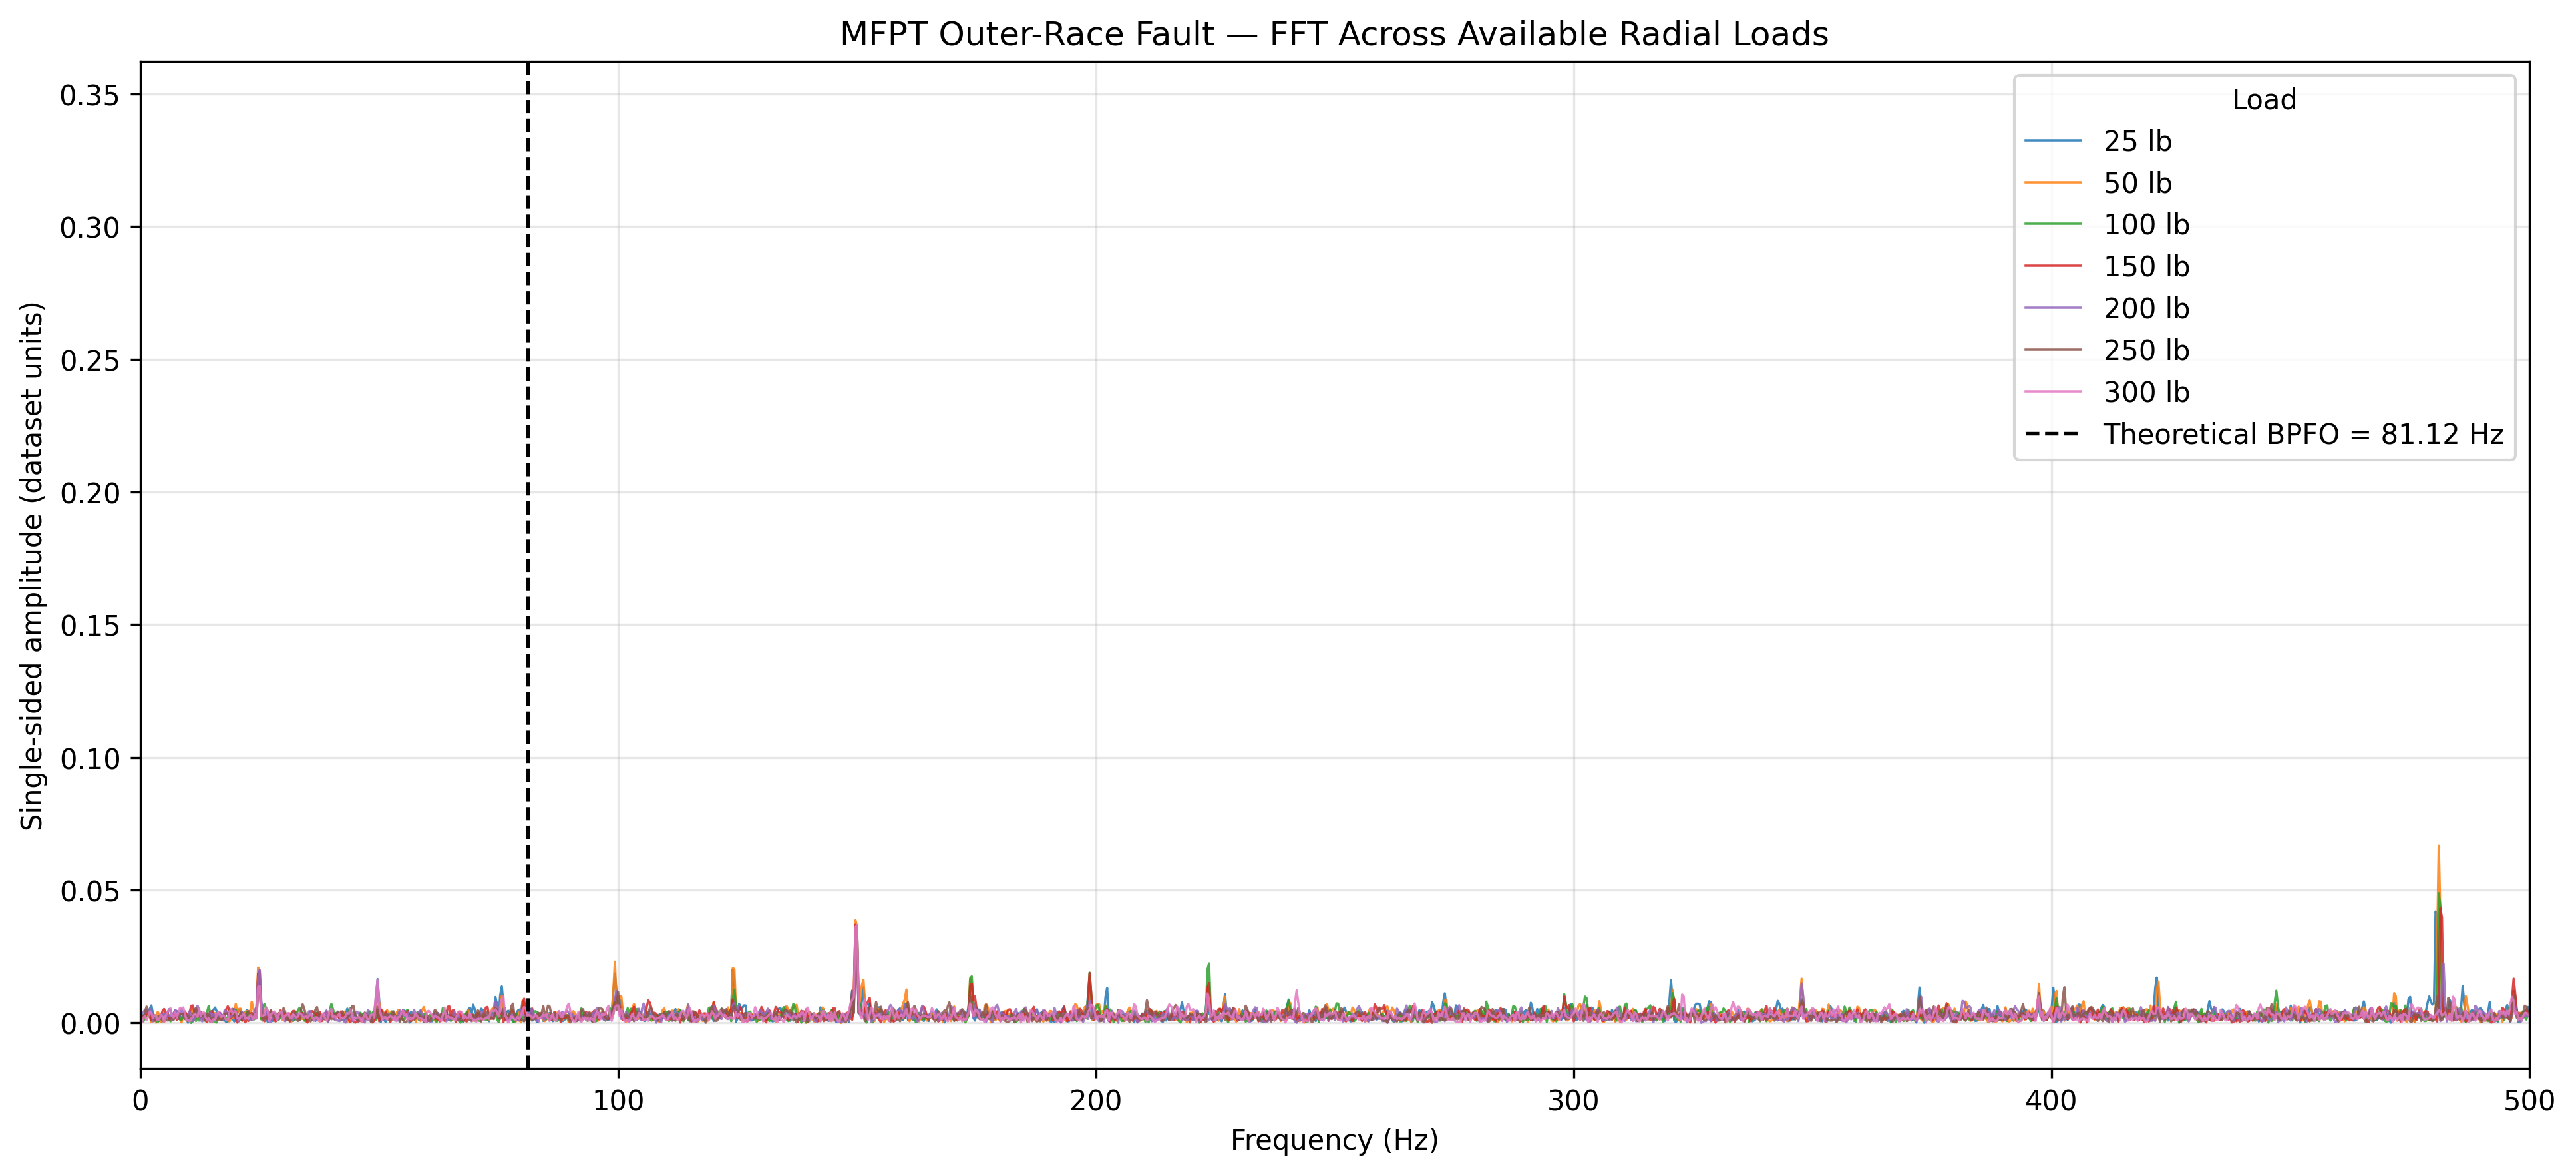
\includegraphics[width=0.60\columnwidth]{figures/figure_6.png}
\captionof{figure}{MFPT outer-race fault: FFT across radial loads.}
\label{fig:m1b2}
\end{minipage}
\end{center}
\vspace{2pt}

\begin{center}
\begin{minipage}{\columnwidth}
\centering
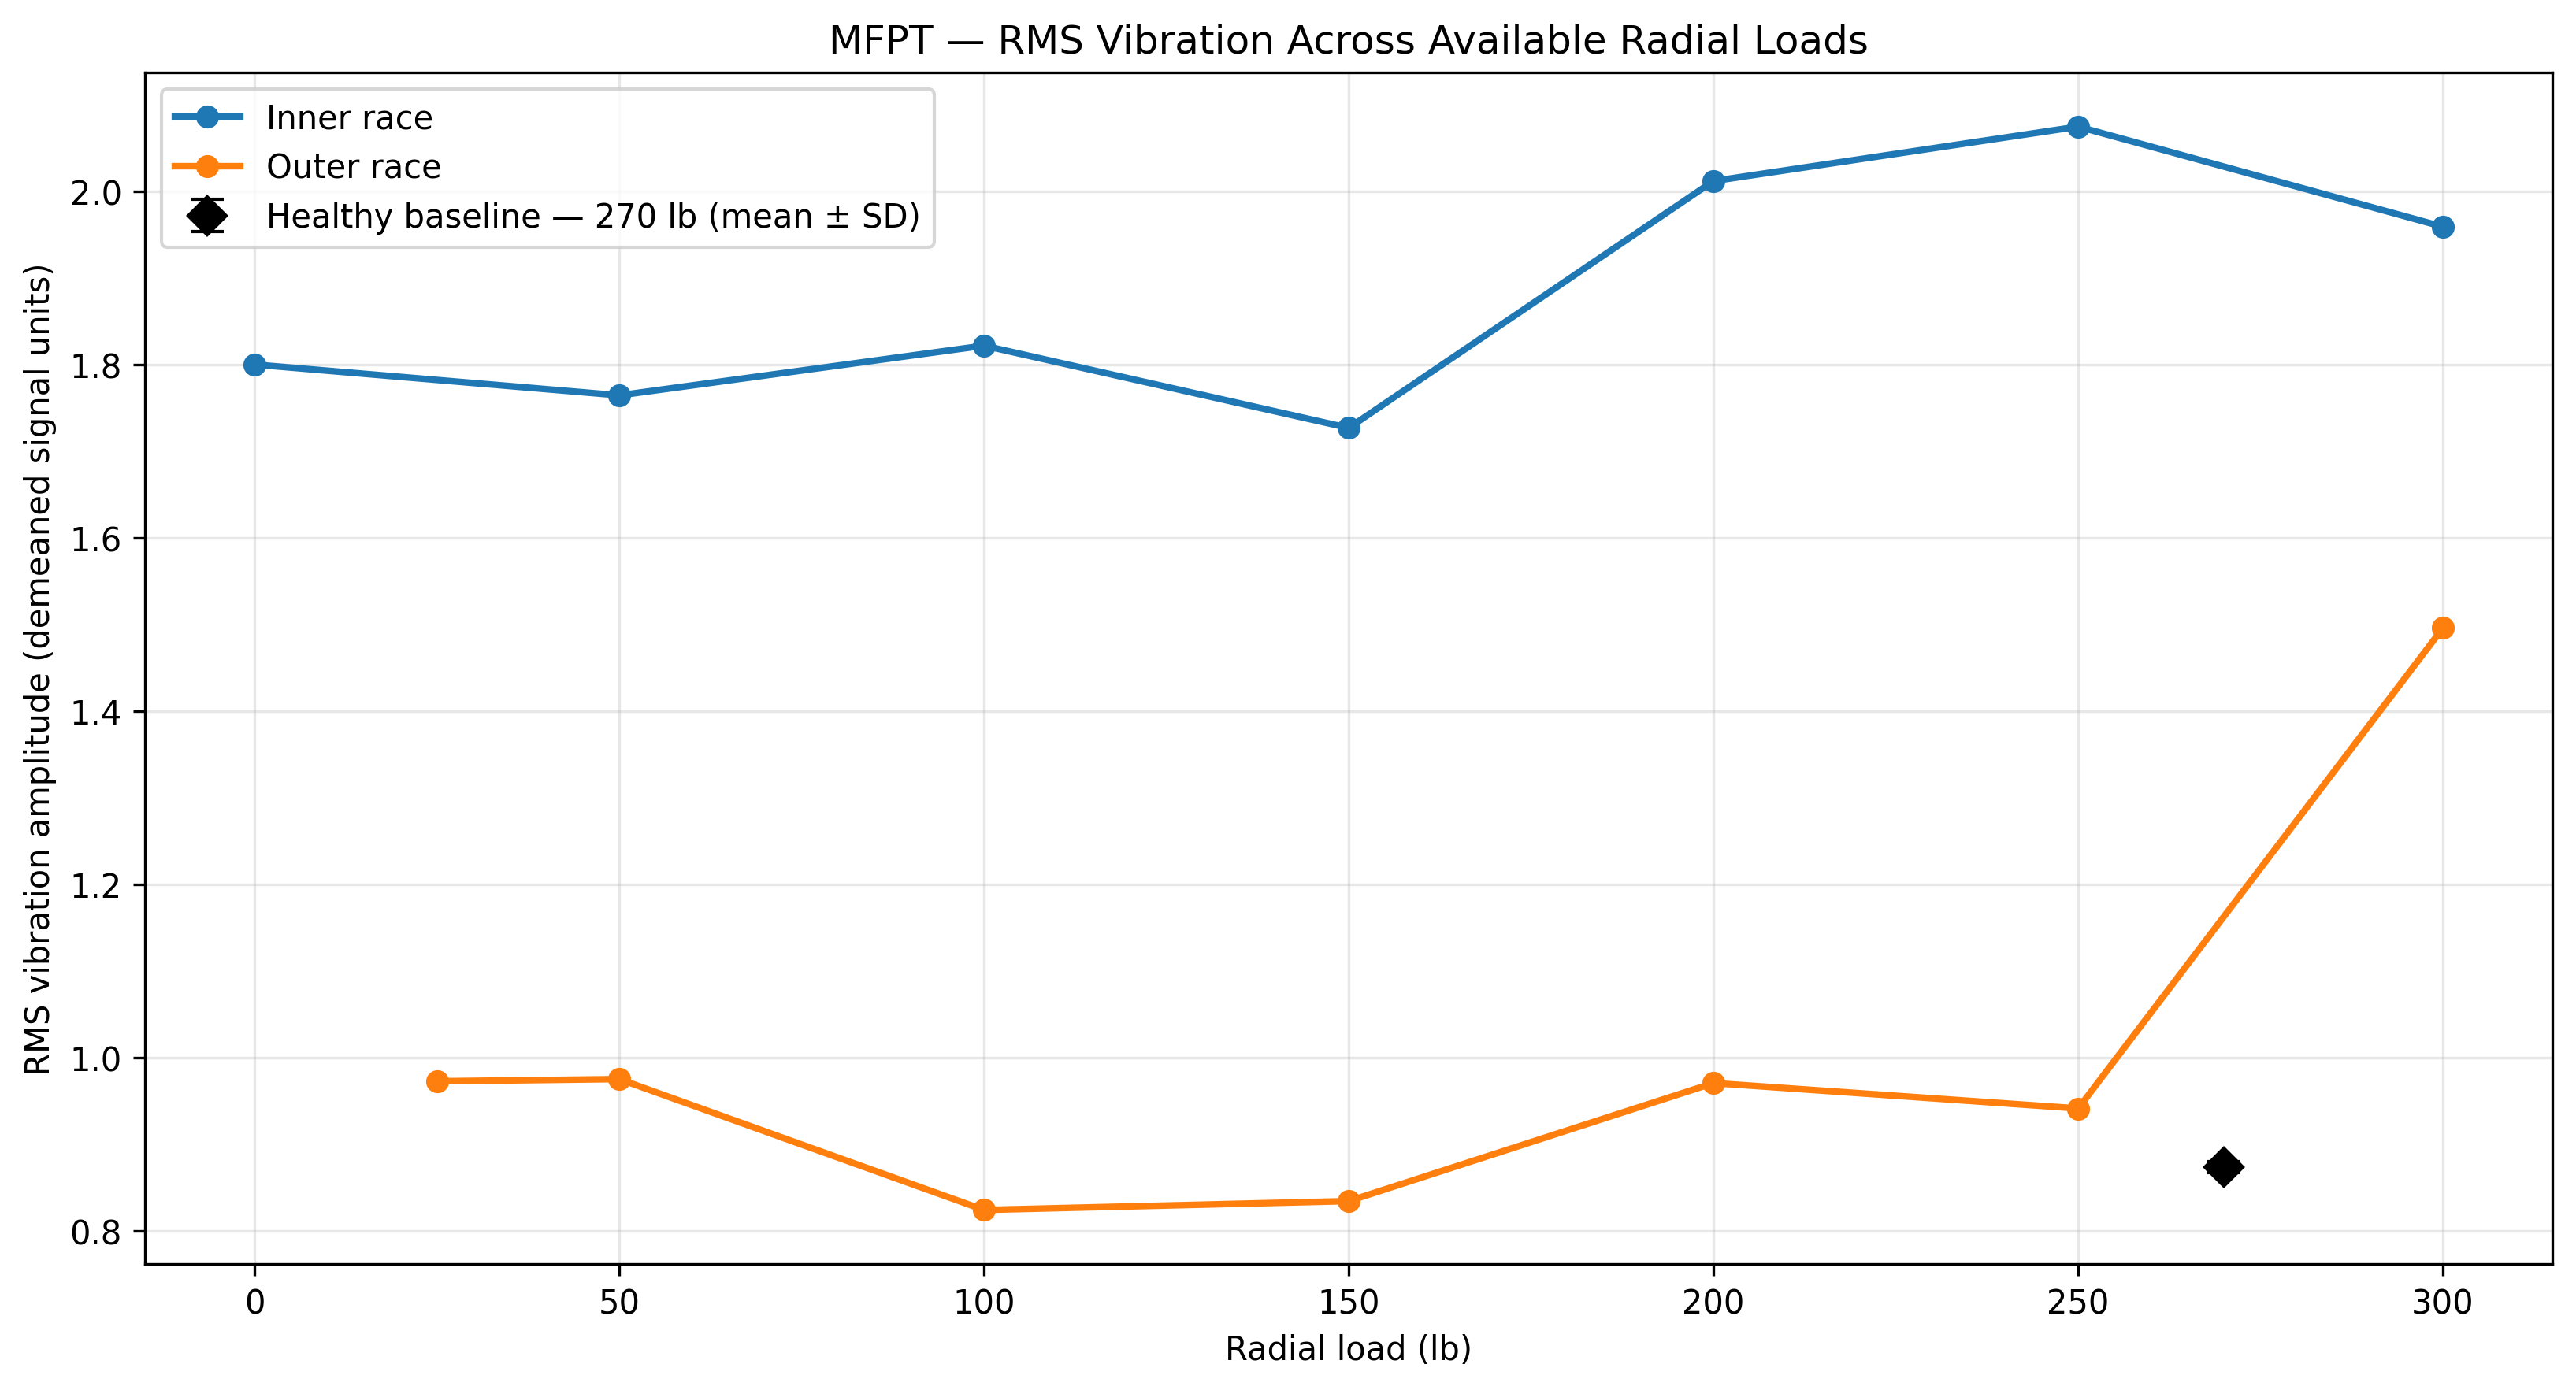
\includegraphics[width=0.60\columnwidth]{figures/figure_7.png}
\captionof{figure}{MFPT RMS vibration amplitude across radial loads.}
\label{fig:m1b3}
\end{minipage}
\end{center}
 % Member 1
}

% ===========================================================================
% Acknowledgment and Author Contributions
% Owner: All
% ===========================================================================
\section*{Acknowledgment}
The authors thank the course faculty for the DSP lecture material on
filter design, Fourier analysis and quantization that this work builds on.

\section*{Author Contributions}
\textbf{Member 1} curated the multi-load CWRU and MFPT datasets, formulated
the discrete-time damped exponential fault model, and implemented kinematic
slip-tolerant frequency tracking. \textbf{Member 2} designed the
Kurtosis-guided resonance selection pipeline, implemented the Kaiser FIR and
bilinear-transform Butterworth cascade-SOS IIR filters, and performed
pole--zero and group-delay analyses. \textbf{Member 3} developed the Hilbert
transform squared-envelope demodulator, calibrated the windowed FFT Squared
Envelope Spectrum, and implemented the CA-CFAR and Median--MAD adaptive
spectral thresholding algorithms. \textbf{Member 4} conducted the multi-load
quantitative benchmarking, evaluated fixed-point quantization feasibility, and
led the integration of the manuscript. All authors reviewed and approved the
final manuscript.

% ===========================================================================
% Bibliography
% Owner: All
% ===========================================================================
\begin{thebibliography}{9}

\bibitem{randall2011}
R.~B. Randall and J.~Antoni, ``Rolling element bearing diagnostics---A
tutorial,'' \emph{Mech. Syst. Signal Process.}, vol.~25, no.~2, pp.~485--520,
2011.

\bibitem{kim2020}
S.~Kim \emph{et al.}, ``Diagnostics 101: A tutorial for fault diagnostics of
rolling element bearing using envelope analysis in MATLAB,'' \emph{Appl. Sci.},
vol.~10, no.~20, p.~7302, 2020.

\bibitem{antoni2007}
J.~Antoni, ``Fast computation of the kurtogram for the detection of transient
faults,'' \emph{Mech. Syst. Signal Process.}, vol.~21, no.~1, pp.~108--124,
2007.

\bibitem{smith2015}
W.~A. Smith and R.~B. Randall, ``Rolling element bearing diagnostics using the
Case Western Reserve University data: A benchmark study,'' \emph{Mech. Syst.
Signal Process.}, vol.~64--65, pp.~100--131, 2015.

\bibitem{oppenheim}
A.~V. Oppenheim and R.~W. Schafer, \emph{Discrete-Time Signal Processing},
3rd~ed. Upper Saddle River, NJ, USA: Prentice Hall, 2009.

\bibitem{proakis}
J.~G. Proakis and D.~G. Manolakis, \emph{Digital Signal Processing: Principles,
Algorithms and Applications}, 4th~ed. Upper Saddle River, NJ, USA: Pearson,
2006.

\bibitem{harris}
F.~J. Harris, ``On the use of windows for harmonic analysis with the discrete
Fourier transform,'' \emph{Proc. IEEE}, vol.~66, no.~1, pp.~51--83, 1978.

\bibitem{finn}
H.~M. Finn and R.~S. Johnson, ``Adaptive detection mode with threshold control
as a function of spatially sampled clutter-level estimates,'' \emph{RCA Rev.},
vol.~29, pp.~414--464, 1968.

\bibitem{rousseeuw}
P.~J. Rousseeuw and C.~Croux, ``Alternatives to the median absolute
deviation,'' \emph{J. Amer. Statist. Assoc.}, vol.~88, no.~424, pp.~1273--1283,
1993.

\end{thebibliography}


\end{document}
